\documentclass[1p]{elsarticle_modified}
%\bibliographystyle{elsarticle-num}

%\usepackage[colorlinks]{hyperref}
%\usepackage{abbrmath_seonhwa} %\Abb, \Ascr, \Acal ,\Abf, \Afrak
\usepackage{amsfonts}
\usepackage{amssymb}
\usepackage{amsmath}
\usepackage{amsthm}
\usepackage{scalefnt}
\usepackage{amsbsy}
\usepackage{kotex}
\usepackage{caption}
\usepackage{subfig}
\usepackage{color}
\usepackage{graphicx}
\usepackage{xcolor} %% white, black, red, green, blue, cyan, magenta, yellow
\usepackage{float}
\usepackage{setspace}
\usepackage{hyperref}

\usepackage{tikz}
\usetikzlibrary{arrows}

\usepackage{multirow}
\usepackage{array} % fixed length table
\usepackage{hhline}

%%%%%%%%%%%%%%%%%%%%%
\makeatletter
\renewcommand*\env@matrix[1][\arraystretch]{%
	\edef\arraystretch{#1}%
	\hskip -\arraycolsep
	\let\@ifnextchar\new@ifnextchar
	\array{*\c@MaxMatrixCols c}}
\makeatother %https://tex.stackexchange.com/questions/14071/how-can-i-increase-the-line-spacing-in-a-matrix
%%%%%%%%%%%%%%%

\usepackage[normalem]{ulem}

\newcommand{\msout}[1]{\ifmmode\text{\sout{\ensuremath{#1}}}\else\sout{#1}\fi}
%SOURCE: \msout is \stkout macro in https://tex.stackexchange.com/questions/20609/strikeout-in-math-mode

\newcommand{\cancel}[1]{
	\ifmmode
	{\color{red}\msout{#1}}
	\else
	{\color{red}\sout{#1}}
	\fi
}

\newcommand{\add}[1]{
	{\color{blue}\uwave{#1}}
}

\newcommand{\replace}[2]{
	\ifmmode
	{\color{red}\msout{#1}}{\color{blue}\uwave{#2}}
	\else
	{\color{red}\sout{#1}}{\color{blue}\uwave{#2}}
	\fi
}

\newcommand{\Sol}{\mathcal{S}} %segment
\newcommand{\D}{D} %diagram
\newcommand{\A}{\mathcal{A}} %arc


%%%%%%%%%%%%%%%%%%%%%%%%%%%%%5 test

\def\sl{\operatorname{\textup{SL}}(2,\Cbb)}
\def\psl{\operatorname{\textup{PSL}}(2,\Cbb)}
\def\quan{\mkern 1mu \triangleright \mkern 1mu}

\theoremstyle{definition}
\newtheorem{thm}{Theorem}[section]
\newtheorem{prop}[thm]{Proposition}
\newtheorem{lem}[thm]{Lemma}
\newtheorem{ques}[thm]{Question}
\newtheorem{cor}[thm]{Corollary}
\newtheorem{defn}[thm]{Definition}
\newtheorem{exam}[thm]{Example}
\newtheorem{rmk}[thm]{Remark}
\newtheorem{alg}[thm]{Algorithm}

\newcommand{\I}{\sqrt{-1}}
\begin{document}

%\begin{frontmatter}
%
%\title{Boundary parabolic representations of knots up to 8 crossings}
%
%%% Group authors per affiliation:
%\author{Yunhi Cho} 
%\address{Department of Mathematics, University of Seoul, Seoul, Korea}
%\ead{yhcho@uos.ac.kr}
%
%
%\author{Seonhwa Kim} %\fnref{s_kim}}
%\address{Center for Geometry and Physics, Institute for Basic Science, Pohang, 37673, Korea}
%\ead{ryeona17@ibs.re.kr}
%
%\author{Hyuk Kim}
%\address{Department of Mathematical Sciences, Seoul National University, Seoul 08826, Korea}
%\ead{hyukkim@snu.ac.kr}
%
%\author{Seokbeom Yoon}
%\address{Department of Mathematical Sciences, Seoul National University, Seoul, 08826,  Korea}
%\ead{sbyoon15@snu.ac.kr}
%
%\begin{abstract}
%We find all boundary parabolic representation of knots up to 8 crossings.
%
%\end{abstract}
%\begin{keyword}
%    \MSC[2010] 57M25 
%\end{keyword}
%
%\end{frontmatter}

%\linenumbers
%\tableofcontents
%
\newcommand\colored[1]{\textcolor{white}{\rule[-0.35ex]{0.8em}{1.4ex}}\kern-0.8em\color{red} #1}%
%\newcommand\colored[1]{\textcolor{white}{ #1}\kern-2.17ex	\textcolor{white}{ #1}\kern-1.81ex	\textcolor{white}{ #1}\kern-2.15ex\color{red}#1	}

{\Large $\underline{12a_{0976}~(K12a_{0976})}$}

\setlength{\tabcolsep}{10pt}
\renewcommand{\arraystretch}{1.6}
\vspace{1cm}\begin{tabular}{m{100pt}>{\centering\arraybackslash}m{274pt}}
\multirow{5}{120pt}{
	\centering
	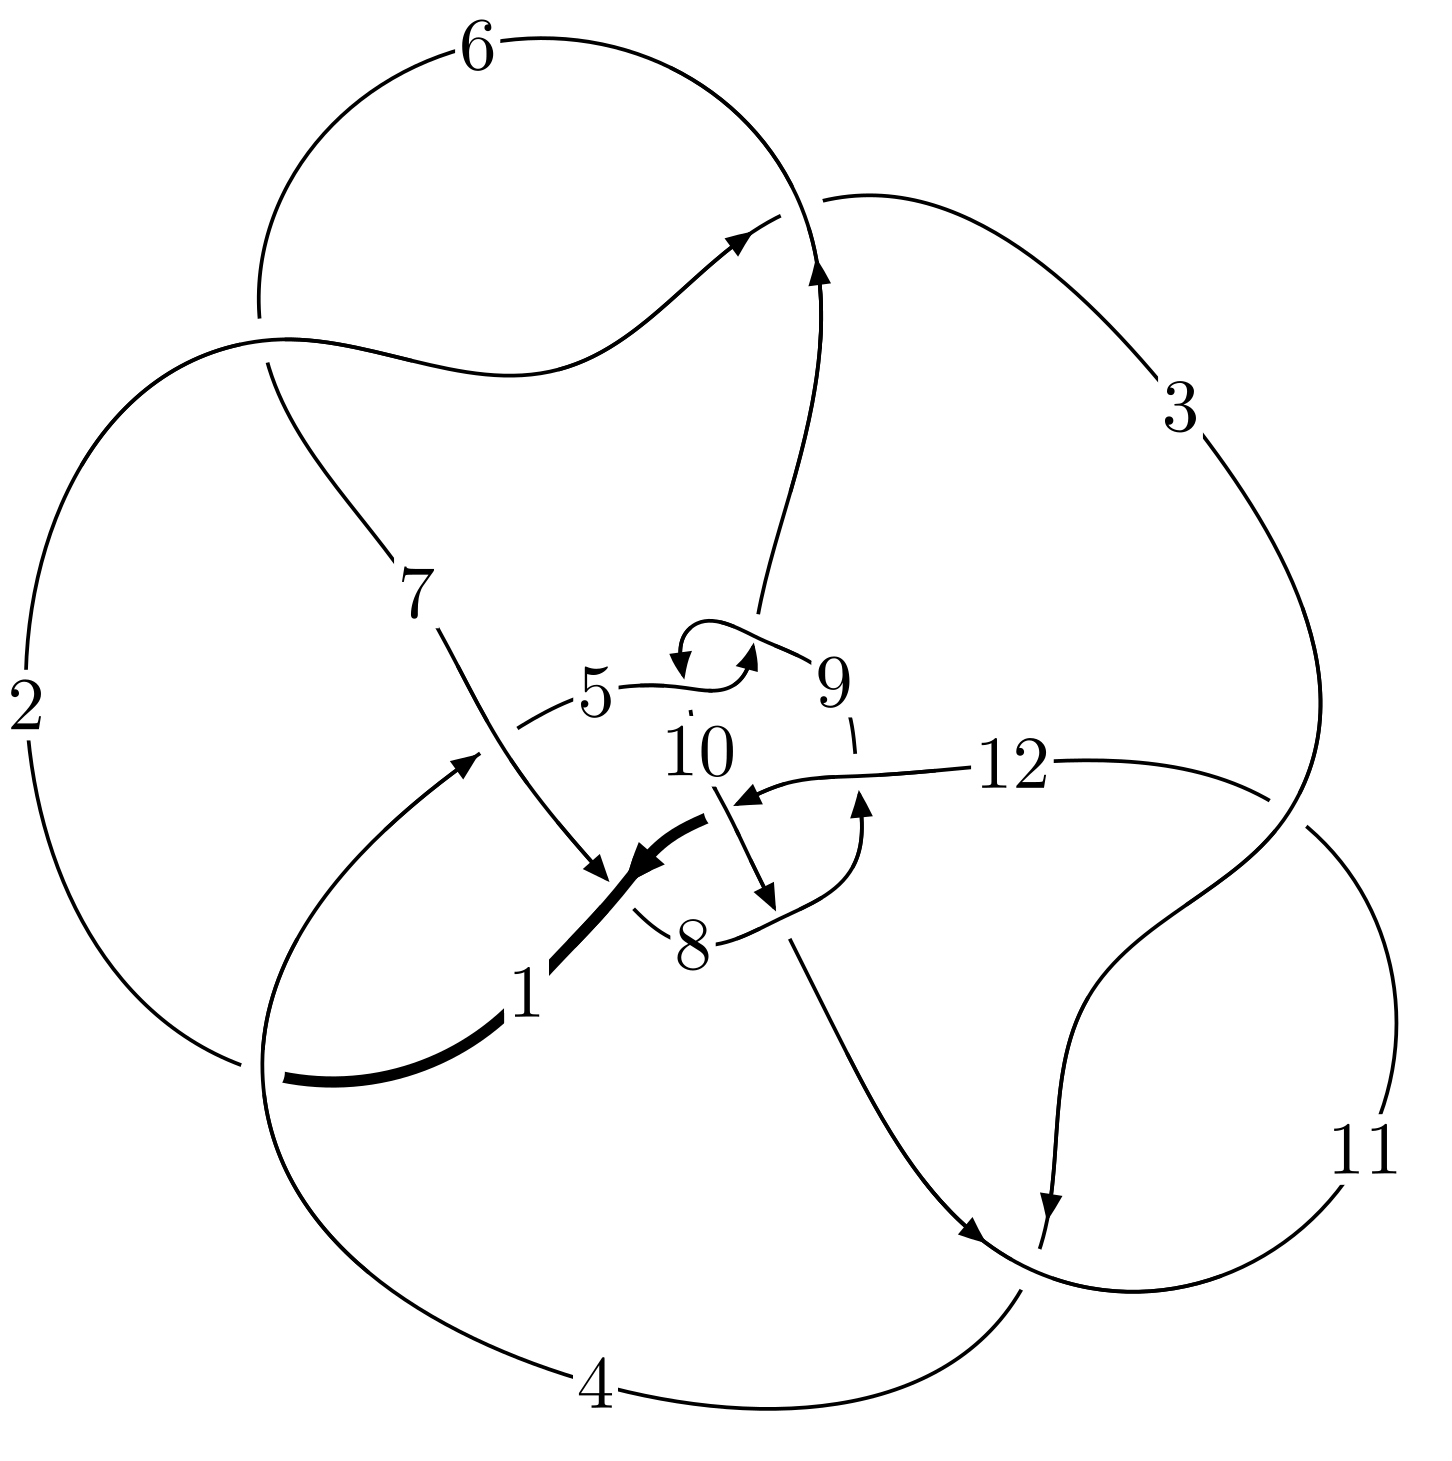
\includegraphics[width=112pt]{../../../GIT/diagram.site/Diagrams/png/1777_12a_0976.png}\\
\ \ \ A knot diagram\footnotemark}&
\allowdisplaybreaks
\textbf{Linearized knot diagam} \\
\cline{2-2}
 &
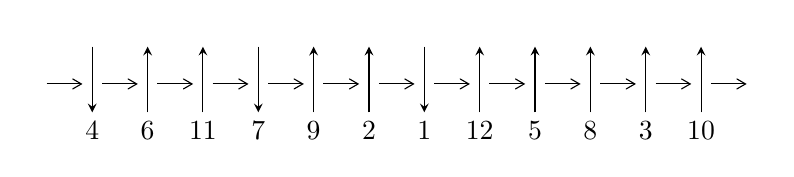
\begin{tikzpicture}[x=20pt, y=17pt]
	% nodes
	\node (C0) at (0, 0) {};
	\node (C1) at (1, 0) {};
	\node (C1U) at (1, +1) {};
	\node (C1D) at (1, -1) {4};

	\node (C2) at (2, 0) {};
	\node (C2U) at (2, +1) {};
	\node (C2D) at (2, -1) {6};

	\node (C3) at (3, 0) {};
	\node (C3U) at (3, +1) {};
	\node (C3D) at (3, -1) {11};

	\node (C4) at (4, 0) {};
	\node (C4U) at (4, +1) {};
	\node (C4D) at (4, -1) {7};

	\node (C5) at (5, 0) {};
	\node (C5U) at (5, +1) {};
	\node (C5D) at (5, -1) {9};

	\node (C6) at (6, 0) {};
	\node (C6U) at (6, +1) {};
	\node (C6D) at (6, -1) {2};

	\node (C7) at (7, 0) {};
	\node (C7U) at (7, +1) {};
	\node (C7D) at (7, -1) {1};

	\node (C8) at (8, 0) {};
	\node (C8U) at (8, +1) {};
	\node (C8D) at (8, -1) {12};

	\node (C9) at (9, 0) {};
	\node (C9U) at (9, +1) {};
	\node (C9D) at (9, -1) {5};

	\node (C10) at (10, 0) {};
	\node (C10U) at (10, +1) {};
	\node (C10D) at (10, -1) {8};

	\node (C11) at (11, 0) {};
	\node (C11U) at (11, +1) {};
	\node (C11D) at (11, -1) {3};

	\node (C12) at (12, 0) {};
	\node (C12U) at (12, +1) {};
	\node (C12D) at (12, -1) {10};
	\node (C13) at (13, 0) {};

	% arrows
	\draw[->,>={angle 60}]
	(C0) edge (C1) (C1) edge (C2) (C2) edge (C3) (C3) edge (C4) (C4) edge (C5) (C5) edge (C6) (C6) edge (C7) (C7) edge (C8) (C8) edge (C9) (C9) edge (C10) (C10) edge (C11) (C11) edge (C12) (C12) edge (C13) ;	\draw[->,>=stealth]
	(C1U) edge (C1D) (C2D) edge (C2U) (C3D) edge (C3U) (C4U) edge (C4D) (C5D) edge (C5U) (C6D) edge (C6U) (C7U) edge (C7D) (C8D) edge (C8U) (C9D) edge (C9U) (C10D) edge (C10U) (C11D) edge (C11U) (C12D) edge (C12U) ;
	\end{tikzpicture} \\
\hhline{~~} \\& 
\textbf{Solving Sequence} \\ \cline{2-2} 
 &
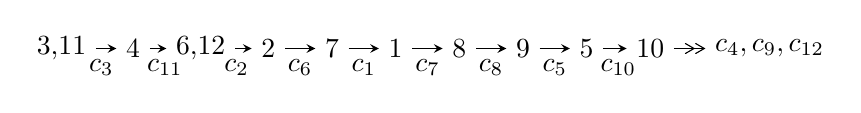
\begin{tikzpicture}[x=23pt, y=7pt]
	% node
	\node (A0) at (-1/8, 0) {3,11};
	\node (A1) at (1, 0) {4};
	\node (A2) at (33/16, 0) {6,12};
	\node (A3) at (25/8, 0) {2};
	\node (A4) at (33/8, 0) {7};
	\node (A5) at (41/8, 0) {1};
	\node (A6) at (49/8, 0) {8};
	\node (A7) at (57/8, 0) {9};
	\node (A8) at (65/8, 0) {5};
	\node (A9) at (73/8, 0) {10};
	\node (C1) at (1/2, -1) {$c_{3}$};
	\node (C2) at (3/2, -1) {$c_{11}$};
	\node (C3) at (21/8, -1) {$c_{2}$};
	\node (C4) at (29/8, -1) {$c_{6}$};
	\node (C5) at (37/8, -1) {$c_{1}$};
	\node (C6) at (45/8, -1) {$c_{7}$};
	\node (C7) at (53/8, -1) {$c_{8}$};
	\node (C8) at (61/8, -1) {$c_{5}$};
	\node (C9) at (69/8, -1) {$c_{10}$};
	\node (A10) at (11, 0) {$c_{4},c_{9},c_{12}$};

	% edge
	\draw[->,>=stealth]	
	(A0) edge (A1) (A1) edge (A2) (A2) edge (A3) (A3) edge (A4) (A4) edge (A5) (A5) edge (A6) (A6) edge (A7) (A7) edge (A8) (A8) edge (A9) ;
	\draw[->>,>={angle 60}]	
	(A9) edge (A10);
\end{tikzpicture} \\ 

\end{tabular} \\

\footnotetext{
The image of knot diagram is generated by the software ``\textbf{Draw programme}" developed by Andrew Bartholomew(\url{http://www.layer8.co.uk/maths/draw/index.htm\#Running-draw}), where we modified some parts for our purpose(\url{https://github.com/CATsTAILs/LinksPainter}).
}\phantom \\ \newline 
\centering \textbf{Ideals for irreducible components\footnotemark of $X_{\text{par}}$} 
 
\begin{align*}
I^u_{1}&=\langle 
-9.36792\times10^{27} u^{40}+8.13492\times10^{26} u^{39}+\cdots+1.40941\times10^{28} b+7.10735\times10^{27},\\
\phantom{I^u_{1}}&\phantom{= \langle  }-7.39544\times10^{27} u^{40}+5.79824\times10^{27} u^{39}+\cdots+4.69805\times10^{27} a-1.57638\times10^{28},\;u^{41}- u^{40}+\cdots+16 u-4\rangle \\
I^u_{2}&=\langle 
3.76586\times10^{963} u^{151}+1.26628\times10^{964} u^{150}+\cdots+6.29219\times10^{964} b-9.83778\times10^{965},\\
\phantom{I^u_{2}}&\phantom{= \langle  }3.81143\times10^{966} u^{151}+1.59111\times10^{967} u^{150}+\cdots+7.99108\times10^{966} a-5.06361\times10^{967},\\
\phantom{I^u_{2}}&\phantom{= \langle  }u^{152}+4 u^{151}+\cdots+5344 u+127\rangle \\
I^u_{3}&=\langle 
-4 u^{15}-2 u^{14}+\cdots+b+11,\;4 u^{15}+25 u^{14}+\cdots+3 a+48,\;u^{16}+u^{15}+\cdots-3 u+3\rangle \\
I^u_{4}&=\langle 
1.46396\times10^{31} u^{35}-5.32684\times10^{31} u^{34}+\cdots+6.50328\times10^{30} b-1.74691\times10^{32},\\
\phantom{I^u_{4}}&\phantom{= \langle  }2.40645\times10^{32} u^{35}-8.53847\times10^{32} u^{34}+\cdots+1.30066\times10^{31} a+2.12996\times10^{33},\;u^{36}-5 u^{35}+\cdots-24 u+4\rangle \\
\\
I^v_{1}&=\langle 
a,\;b+v,\;v^2- v+1\rangle \\
\end{align*}
\raggedright * 5 irreducible components of $\dim_{\mathbb{C}}=0$, with total 247 representations.\\
\footnotetext{All coefficients of polynomials are rational numbers. But the coefficients are sometimes approximated in decimal forms when there is not enough margin.}
\newpage
\renewcommand{\arraystretch}{1}
\centering \section*{I. $I^u_{1}= \langle -9.37\times10^{27} u^{40}+8.13\times10^{26} u^{39}+\cdots+1.41\times10^{28} b+7.11\times10^{27},\;-7.40\times10^{27} u^{40}+5.80\times10^{27} u^{39}+\cdots+4.70\times10^{27} a-1.58\times10^{28},\;u^{41}- u^{40}+\cdots+16 u-4 \rangle$}
\flushleft \textbf{(i) Arc colorings}\\
\begin{tabular}{m{7pt} m{180pt} m{7pt} m{180pt} }
\flushright $a_{3}=$&$\begin{pmatrix}1\\0\end{pmatrix}$ \\
\flushright $a_{11}=$&$\begin{pmatrix}0\\u\end{pmatrix}$ \\
\flushright $a_{4}=$&$\begin{pmatrix}1\\- u^2\end{pmatrix}$ \\
\flushright $a_{6}=$&$\begin{pmatrix}1.57415 u^{40}-1.23418 u^{39}+\cdots-15.1906 u+3.35539\\0.664667 u^{40}-0.0577185 u^{39}+\cdots-1.60599 u-0.504277\end{pmatrix}$ \\
\flushright $a_{12}=$&$\begin{pmatrix}u\\u\end{pmatrix}$ \\
\flushright $a_{2}=$&$\begin{pmatrix}-1.08851 u^{40}+1.67936 u^{39}+\cdots+22.4118 u-4.32639\\-0.617870 u^{40}+0.662158 u^{39}+\cdots+8.27389 u-1.88526\end{pmatrix}$ \\
\flushright $a_{7}=$&$\begin{pmatrix}1.85378 u^{40}-2.97661 u^{39}+\cdots-44.3273 u+10.8054\\1.40222 u^{40}-1.50444 u^{39}+\cdots-19.8467 u+4.01319\end{pmatrix}$ \\
\flushright $a_{1}=$&$\begin{pmatrix}-0.478088 u^{40}+1.13344 u^{39}+\cdots+16.8780 u-3.84825\\-0.165222 u^{40}+0.391963 u^{39}+\cdots+6.86426 u-2.14327\end{pmatrix}$ \\
\flushright $a_{8}=$&$\begin{pmatrix}0.0710383 u^{40}+0.170175 u^{39}+\cdots+1.05064 u+1.10767\\-0.763787 u^{40}+1.64557 u^{39}+\cdots+24.2806 u-6.20023\end{pmatrix}$ \\
\flushright $a_{9}=$&$\begin{pmatrix}1.10180 u^{40}-0.871388 u^{39}+\cdots-12.5378 u+3.66997\\0.266978 u^{40}+0.604011 u^{39}+\cdots+10.6921 u-3.63794\end{pmatrix}$ \\
\flushright $a_{5}=$&$\begin{pmatrix}1.34374 u^{40}+0.0709335 u^{39}+\cdots-1.23170 u-1.05183\\-0.206321 u^{40}+0.857204 u^{39}+\cdots+6.30360 u-1.57219\end{pmatrix}$ \\
\flushright $a_{10}=$&$\begin{pmatrix}0.312866 u^{40}-0.741479 u^{39}+\cdots-10.0138 u+1.70498\\0.383904 u^{40}-0.571305 u^{39}+\cdots-8.96313 u+2.81265\end{pmatrix}$\\&\end{tabular}
\flushleft \textbf{(ii) Obstruction class $= -1$}\\~\\
\flushleft \textbf{(iii) Cusp Shapes $= -\frac{3034752482244072423566867802}{1174511702315840550034715077} u^{40}-\frac{142264458706085874111596356}{1174511702315840550034715077} u^{39}+\cdots-\frac{38859810324958590784929033798}{1174511702315840550034715077} u+\frac{26045816357872276194720333966}{1174511702315840550034715077}$}\\~\\
\newpage\renewcommand{\arraystretch}{1}
\flushleft \textbf{(iv) u-Polynomials at the component}\newline \\
\begin{tabular}{m{50pt}|m{274pt}}
Crossings & \hspace{64pt}u-Polynomials at each crossing \\
\hline $$\begin{aligned}c_{1},c_{4}\end{aligned}$$&$\begin{aligned}
&u^{41}- u^{40}+\cdots+5 u-1
\end{aligned}$\\
\hline $$\begin{aligned}c_{2},c_{6}\end{aligned}$$&$\begin{aligned}
&u^{41}-18 u^{40}+\cdots+3856 u-272
\end{aligned}$\\
\hline $$\begin{aligned}c_{3},c_{5},c_{9}\\c_{11}\end{aligned}$$&$\begin{aligned}
&u^{41}- u^{40}+\cdots+16 u-4
\end{aligned}$\\
\hline $$\begin{aligned}c_{7}\end{aligned}$$&$\begin{aligned}
&u^{41}-35 u^{40}+\cdots+9437184 u-524288
\end{aligned}$\\
\hline $$\begin{aligned}c_{8}\end{aligned}$$&$\begin{aligned}
&u^{41}-28 u^{40}+\cdots+146856 u-11968
\end{aligned}$\\
\hline $$\begin{aligned}c_{10},c_{12}\end{aligned}$$&$\begin{aligned}
&u^{41}+u^{40}+\cdots- u-1
\end{aligned}$\\
\hline
\end{tabular}\\~\\
\newpage\renewcommand{\arraystretch}{1}
\flushleft \textbf{(v) Riley Polynomials at the component}\newline \\
\begin{tabular}{m{50pt}|m{274pt}}
Crossings & \hspace{64pt}Riley Polynomials at each crossing \\
\hline $$\begin{aligned}c_{1},c_{4}\end{aligned}$$&$\begin{aligned}
&y^{41}-17 y^{40}+\cdots+47 y-1
\end{aligned}$\\
\hline $$\begin{aligned}c_{2},c_{6}\end{aligned}$$&$\begin{aligned}
&y^{41}+30 y^{40}+\cdots+474496 y-73984
\end{aligned}$\\
\hline $$\begin{aligned}c_{3},c_{5},c_{9}\\c_{11}\end{aligned}$$&$\begin{aligned}
&y^{41}+29 y^{40}+\cdots+208 y^2-16
\end{aligned}$\\
\hline $$\begin{aligned}c_{7}\end{aligned}$$&$\begin{aligned}
&y^{41}+9 y^{40}+\cdots+1649267441664 y-274877906944
\end{aligned}$\\
\hline $$\begin{aligned}c_{8}\end{aligned}$$&$\begin{aligned}
&y^{41}-8 y^{40}+\cdots-428680128 y-143233024
\end{aligned}$\\
\hline $$\begin{aligned}c_{10},c_{12}\end{aligned}$$&$\begin{aligned}
&y^{41}+7 y^{40}+\cdots+y-1
\end{aligned}$\\
\hline
\end{tabular}\\~\\
\newpage\flushleft \textbf{(vi) Complex Volumes and Cusp Shapes}
$$\begin{array}{c|c|c}  
\text{Solutions to }I^u_{1}& \I (\text{vol} + \sqrt{-1}CS) & \text{Cusp shape}\\
 \hline 
\begin{aligned}
u &= \phantom{-}0.355254 + 0.957355 I \\
a &= -0.943476 - 0.548882 I \\
b &= -0.725619 + 0.128110 I\end{aligned}
 & -1.17120 + 5.93299 I & \phantom{-}4.82099 - 13.25602 I \\ \hline\begin{aligned}
u &= \phantom{-}0.355254 - 0.957355 I \\
a &= -0.943476 + 0.548882 I \\
b &= -0.725619 - 0.128110 I\end{aligned}
 & -1.17120 - 5.93299 I & \phantom{-}4.82099 + 13.25602 I \\ \hline\begin{aligned}
u &= \phantom{-}0.182709 + 0.955930 I \\
a &= \phantom{-}0.59415 - 2.33874 I \\
b &= -0.78874 - 1.31820 I\end{aligned}
 & -3.41939 - 0.61188 I & -4.06956 + 3.27847 I \\ \hline\begin{aligned}
u &= \phantom{-}0.182709 - 0.955930 I \\
a &= \phantom{-}0.59415 + 2.33874 I \\
b &= -0.78874 + 1.31820 I\end{aligned}
 & -3.41939 + 0.61188 I & -4.06956 - 3.27847 I \\ \hline\begin{aligned}
u &= \phantom{-}0.312542 + 1.016120 I \\
a &= -0.170843 + 0.707646 I \\
b &= \phantom{-}0.887449 + 0.244109 I\end{aligned}
 & -2.15556 + 2.75564 I & \phantom{-}2.75882 - 3.02176 I \\ \hline\begin{aligned}
u &= \phantom{-}0.312542 - 1.016120 I \\
a &= -0.170843 - 0.707646 I \\
b &= \phantom{-}0.887449 - 0.244109 I\end{aligned}
 & -2.15556 - 2.75564 I & \phantom{-}2.75882 + 3.02176 I \\ \hline\begin{aligned}
u &= -0.829768 + 0.414937 I \\
a &= \phantom{-}0.401759 + 0.549858 I \\
b &= -0.795790 + 0.091594 I\end{aligned}
 & \phantom{-}3.84345 + 4.13042 I & \phantom{-}11.18782 - 2.61819 I \\ \hline\begin{aligned}
u &= -0.829768 - 0.414937 I \\
a &= \phantom{-}0.401759 - 0.549858 I \\
b &= -0.795790 - 0.091594 I\end{aligned}
 & \phantom{-}3.84345 - 4.13042 I & \phantom{-}11.18782 + 2.61819 I \\ \hline\begin{aligned}
u &= \phantom{-}1.057050 + 0.246411 I \\
a &= \phantom{-}0.173938 + 0.652642 I \\
b &= -0.417916 + 1.222970 I\end{aligned}
 & \phantom{-}0.36430 - 8.56808 I & \phantom{-}5.99108 + 6.74347 I \\ \hline\begin{aligned}
u &= \phantom{-}1.057050 - 0.246411 I \\
a &= \phantom{-}0.173938 - 0.652642 I \\
b &= -0.417916 - 1.222970 I\end{aligned}
 & \phantom{-}0.36430 + 8.56808 I & \phantom{-}5.99108 - 6.74347 I\\
 \hline 
 \end{array}$$\newpage$$\begin{array}{c|c|c}  
\text{Solutions to }I^u_{1}& \I (\text{vol} + \sqrt{-1}CS) & \text{Cusp shape}\\
 \hline 
\begin{aligned}
u &= \phantom{-}0.282856 + 1.165060 I \\
a &= -0.606099 - 0.167833 I \\
b &= -1.38265 + 0.62746 I\end{aligned}
 & -5.75137 + 3.96802 I & -4.24316 - 1.27024 I \\ \hline\begin{aligned}
u &= \phantom{-}0.282856 - 1.165060 I \\
a &= -0.606099 + 0.167833 I \\
b &= -1.38265 - 0.62746 I\end{aligned}
 & -5.75137 - 3.96802 I & -4.24316 + 1.27024 I \\ \hline\begin{aligned}
u &= -0.765233 + 0.027384 I \\
a &= \phantom{-}0.544878 + 0.272827 I \\
b &= -0.346266 + 1.126520 I\end{aligned}
 & -1.84700 - 2.91345 I & \phantom{-}3.24294 + 4.74634 I \\ \hline\begin{aligned}
u &= -0.765233 - 0.027384 I \\
a &= \phantom{-}0.544878 - 0.272827 I \\
b &= -0.346266 - 1.126520 I\end{aligned}
 & -1.84700 + 2.91345 I & \phantom{-}3.24294 - 4.74634 I \\ \hline\begin{aligned}
u &= -0.355013 + 1.204340 I \\
a &= -0.592249 + 0.345245 I \\
b &= \phantom{-}0.348655 + 0.463430 I\end{aligned}
 & -5.80010 - 0.30487 I & -4.31941 - 0.73616 I \\ \hline\begin{aligned}
u &= -0.355013 - 1.204340 I \\
a &= -0.592249 - 0.345245 I \\
b &= \phantom{-}0.348655 - 0.463430 I\end{aligned}
 & -5.80010 + 0.30487 I & -4.31941 + 0.73616 I \\ \hline\begin{aligned}
u &= -0.357497 + 1.225470 I \\
a &= \phantom{-}0.65659 + 2.23078 I \\
b &= -0.481655 + 1.303690 I\end{aligned}
 & -4.91754 - 10.74480 I & \phantom{-}4.64446 + 9.26386 I \\ \hline\begin{aligned}
u &= -0.357497 - 1.225470 I \\
a &= \phantom{-}0.65659 - 2.23078 I \\
b &= -0.481655 - 1.303690 I\end{aligned}
 & -4.91754 + 10.74480 I & \phantom{-}4.64446 - 9.26386 I \\ \hline\begin{aligned}
u &= \phantom{-}0.198188 + 0.673749 I \\
a &= -1.44436 + 0.31882 I \\
b &= -0.520200 - 0.640823 I\end{aligned}
 & -1.58494 + 6.26446 I & \phantom{-}1.10892 - 8.48549 I \\ \hline\begin{aligned}
u &= \phantom{-}0.198188 - 0.673749 I \\
a &= -1.44436 - 0.31882 I \\
b &= -0.520200 + 0.640823 I\end{aligned}
 & -1.58494 - 6.26446 I & \phantom{-}1.10892 + 8.48549 I\\
 \hline 
 \end{array}$$\newpage$$\begin{array}{c|c|c}  
\text{Solutions to }I^u_{1}& \I (\text{vol} + \sqrt{-1}CS) & \text{Cusp shape}\\
 \hline 
\begin{aligned}
u &= \phantom{-}0.470339 + 0.520796 I \\
a &= \phantom{-}0.949040 - 0.250865 I \\
b &= -0.692863 - 0.570833 I\end{aligned}
 & \phantom{-}1.54510 + 1.18608 I & \phantom{-}8.80668 + 0.32091 I \\ \hline\begin{aligned}
u &= \phantom{-}0.470339 - 0.520796 I \\
a &= \phantom{-}0.949040 + 0.250865 I \\
b &= -0.692863 + 0.570833 I\end{aligned}
 & \phantom{-}1.54510 - 1.18608 I & \phantom{-}8.80668 - 0.32091 I \\ \hline\begin{aligned}
u &= -0.541532 + 0.429703 I \\
a &= \phantom{-}0.798167 - 0.298634 I \\
b &= -0.584304 - 1.023470 I\end{aligned}
 & \phantom{-}0.13834 + 3.71774 I & \phantom{-}8.24552 - 0.59208 I \\ \hline\begin{aligned}
u &= -0.541532 - 0.429703 I \\
a &= \phantom{-}0.798167 + 0.298634 I \\
b &= -0.584304 + 1.023470 I\end{aligned}
 & \phantom{-}0.13834 - 3.71774 I & \phantom{-}8.24552 + 0.59208 I \\ \hline\begin{aligned}
u &= \phantom{-}0.201344 + 1.294790 I \\
a &= -0.60451 + 1.70665 I \\
b &= -0.53100 + 2.37595 I\end{aligned}
 & -7.25907 + 6.02782 I & -24.9299 - 9.4175 I \\ \hline\begin{aligned}
u &= \phantom{-}0.201344 - 1.294790 I \\
a &= -0.60451 - 1.70665 I \\
b &= -0.53100 - 2.37595 I\end{aligned}
 & -7.25907 - 6.02782 I & -24.9299 + 9.4175 I \\ \hline\begin{aligned}
u &= -0.507037 + 1.212430 I \\
a &= \phantom{-}0.94888 + 1.67421 I \\
b &= -0.74687 + 1.42147 I\end{aligned}
 & -8.9112 - 11.8653 I & -2.47418 + 10.59886 I \\ \hline\begin{aligned}
u &= -0.507037 - 1.212430 I \\
a &= \phantom{-}0.94888 - 1.67421 I \\
b &= -0.74687 - 1.42147 I\end{aligned}
 & -8.9112 + 11.8653 I & -2.47418 - 10.59886 I \\ \hline\begin{aligned}
u &= -0.652124 + 1.149880 I \\
a &= -1.07807 - 1.24272 I \\
b &= \phantom{-}0.270848 - 1.313070 I\end{aligned}
 & -7.26445 - 6.58554 I & \phantom{-0.000000 -}0. + 6.24258 I \\ \hline\begin{aligned}
u &= -0.652124 - 1.149880 I \\
a &= -1.07807 + 1.24272 I \\
b &= \phantom{-}0.270848 + 1.313070 I\end{aligned}
 & -7.26445 + 6.58554 I & \phantom{-0.000000 } 0. - 6.24258 I\\
 \hline 
 \end{array}$$\newpage$$\begin{array}{c|c|c}  
\text{Solutions to }I^u_{1}& \I (\text{vol} + \sqrt{-1}CS) & \text{Cusp shape}\\
 \hline 
\begin{aligned}
u &= -0.553913 + 1.274090 I \\
a &= -0.220887 + 0.527421 I \\
b &= -1.392050 + 0.043136 I\end{aligned}
 & -1.6816 - 14.7698 I & \phantom{-0.000000 -}0. + 10.08826 I \\ \hline\begin{aligned}
u &= -0.553913 - 1.274090 I \\
a &= -0.220887 - 0.527421 I \\
b &= -1.392050 - 0.043136 I\end{aligned}
 & -1.6816 + 14.7698 I & \phantom{-0.000000 } 0. - 10.08826 I \\ \hline\begin{aligned}
u &= \phantom{-}0.486851 + 0.244403 I \\
a &= \phantom{-}1.85925 - 0.90732 I \\
b &= -0.273613 - 0.988318 I\end{aligned}
 & \phantom{-}0.022808 - 0.870233 I & \phantom{-}6.94699 + 0.81647 I \\ \hline\begin{aligned}
u &= \phantom{-}0.486851 - 0.244403 I \\
a &= \phantom{-}1.85925 + 0.90732 I \\
b &= -0.273613 + 0.988318 I\end{aligned}
 & \phantom{-}0.022808 + 0.870233 I & \phantom{-}6.94699 - 0.81647 I \\ \hline\begin{aligned}
u &= -0.05192 + 1.46914 I \\
a &= -0.22904 - 1.73436 I \\
b &= -0.21282 - 1.46235 I\end{aligned}
 & -13.31590 + 0.60859 I & \phantom{-0.000000 } 0 \\ \hline\begin{aligned}
u &= -0.05192 - 1.46914 I \\
a &= -0.22904 + 1.73436 I \\
b &= -0.21282 + 1.46235 I\end{aligned}
 & -13.31590 - 0.60859 I & \phantom{-0.000000 } 0 \\ \hline\begin{aligned}
u &= \phantom{-}0.65516 + 1.35458 I \\
a &= -1.01542 + 1.19287 I \\
b &= \phantom{-}0.174557 + 1.168400 I\end{aligned}
 & -8.10806 + 2.31475 I & \phantom{-0.000000 } 0 \\ \hline\begin{aligned}
u &= \phantom{-}0.65516 - 1.35458 I \\
a &= -1.01542 - 1.19287 I \\
b &= \phantom{-}0.174557 - 1.168400 I\end{aligned}
 & -8.10806 - 2.31475 I & \phantom{-0.000000 } 0 \\ \hline\begin{aligned}
u &= \phantom{-}0.70626 + 1.36288 I \\
a &= \phantom{-}0.87484 - 1.51677 I \\
b &= -0.61588 - 1.45307 I\end{aligned}
 & -6.3818 + 21.6497 I & \phantom{-0.000000 } 0 \\ \hline\begin{aligned}
u &= \phantom{-}0.70626 - 1.36288 I \\
a &= \phantom{-}0.87484 + 1.51677 I \\
b &= -0.61588 + 1.45307 I\end{aligned}
 & -6.3818 - 21.6497 I & \phantom{-0.000000 } 0\\
 \hline 
 \end{array}$$\newpage$$\begin{array}{c|c|c}  
\text{Solutions to }I^u_{1}& \I (\text{vol} + \sqrt{-1}CS) & \text{Cusp shape}\\
 \hline 
\begin{aligned}
u &= \phantom{-}0.410975\phantom{ +0.000000I} \\
a &= \phantom{-}1.20694\phantom{ +0.000000I} \\
b &= -0.346533\phantom{ +0.000000I}\end{aligned}
 & \phantom{-}0.911167\phantom{ +0.000000I} & \phantom{-}11.2160\phantom{ +0.000000I}\\
 \hline 
 \end{array}$$\newpage\newpage\renewcommand{\arraystretch}{1}
\centering \section*{II. $I^u_{2}= \langle 3.77\times10^{963} u^{151}+1.27\times10^{964} u^{150}+\cdots+6.29\times10^{964} b-9.84\times10^{965},\;3.81\times10^{966} u^{151}+1.59\times10^{967} u^{150}+\cdots+7.99\times10^{966} a-5.06\times10^{967},\;u^{152}+4 u^{151}+\cdots+5344 u+127 \rangle$}
\flushleft \textbf{(i) Arc colorings}\\
\begin{tabular}{m{7pt} m{180pt} m{7pt} m{180pt} }
\flushright $a_{3}=$&$\begin{pmatrix}1\\0\end{pmatrix}$ \\
\flushright $a_{11}=$&$\begin{pmatrix}0\\u\end{pmatrix}$ \\
\flushright $a_{4}=$&$\begin{pmatrix}1\\- u^2\end{pmatrix}$ \\
\flushright $a_{6}=$&$\begin{pmatrix}-0.476961 u^{151}-1.99111 u^{150}+\cdots-829.800 u+6.33658\\-0.0598497 u^{151}-0.201247 u^{150}+\cdots+601.956 u+15.6349\end{pmatrix}$ \\
\flushright $a_{12}=$&$\begin{pmatrix}u\\u\end{pmatrix}$ \\
\flushright $a_{2}=$&$\begin{pmatrix}-0.550082 u^{151}-1.82843 u^{150}+\cdots+1728.55 u+60.0372\\-0.286239 u^{151}-0.977703 u^{150}+\cdots+1408.59 u+35.6321\end{pmatrix}$ \\
\flushright $a_{7}=$&$\begin{pmatrix}-0.476089 u^{151}-1.67154 u^{150}+\cdots+290.281 u+41.1953\\-0.407293 u^{151}-1.47309 u^{150}+\cdots+1449.28 u+37.6940\end{pmatrix}$ \\
\flushright $a_{1}=$&$\begin{pmatrix}-0.390488 u^{151}-1.29157 u^{150}+\cdots+1219.57 u+48.4380\\-0.0987343 u^{151}-0.315899 u^{150}+\cdots+886.357 u+22.7394\end{pmatrix}$ \\
\flushright $a_{8}=$&$\begin{pmatrix}0.201437 u^{151}+0.956029 u^{150}+\cdots+1264.00 u+65.5938\\-0.0108564 u^{151}-0.0121123 u^{150}+\cdots+553.852 u+14.7828\end{pmatrix}$ \\
\flushright $a_{9}=$&$\begin{pmatrix}0.278529 u^{151}+1.33447 u^{150}+\cdots+1926.73 u+80.7029\\0.0662356 u^{151}+0.366329 u^{150}+\cdots+1216.58 u+29.8919\end{pmatrix}$ \\
\flushright $a_{5}=$&$\begin{pmatrix}-0.421507 u^{151}-1.67481 u^{150}+\cdots-2145.24 u-39.1653\\-0.351584 u^{151}-1.43290 u^{150}+\cdots+101.022 u+4.75533\end{pmatrix}$ \\
\flushright $a_{10}=$&$\begin{pmatrix}-0.475745 u^{151}-1.99625 u^{150}+\cdots-2006.72 u-31.0923\\-0.563910 u^{151}-2.24307 u^{150}+\cdots+90.2285 u+5.33301\end{pmatrix}$\\&\end{tabular}
\flushleft \textbf{(ii) Obstruction class $= -1$}\\~\\
\flushleft \textbf{(iii) Cusp Shapes $= -6.75818 u^{151}-30.4274 u^{150}+\cdots-15015.3 u-319.503$}\\~\\
\newpage\renewcommand{\arraystretch}{1}
\flushleft \textbf{(iv) u-Polynomials at the component}\newline \\
\begin{tabular}{m{50pt}|m{274pt}}
Crossings & \hspace{64pt}u-Polynomials at each crossing \\
\hline $$\begin{aligned}c_{1},c_{4}\end{aligned}$$&$\begin{aligned}
&u^{152}-12 u^{151}+\cdots-8870 u+337
\end{aligned}$\\
\hline $$\begin{aligned}c_{2},c_{6}\end{aligned}$$&$\begin{aligned}
&(u^{76}+8 u^{75}+\cdots+21348 u+1357)^{2}
\end{aligned}$\\
\hline $$\begin{aligned}c_{3},c_{5},c_{9}\\c_{11}\end{aligned}$$&$\begin{aligned}
&u^{152}+4 u^{151}+\cdots+5344 u+127
\end{aligned}$\\
\hline $$\begin{aligned}c_{7}\end{aligned}$$&$\begin{aligned}
&(u^{76}+14 u^{75}+\cdots+18 u+1)^{2}
\end{aligned}$\\
\hline $$\begin{aligned}c_{8}\end{aligned}$$&$\begin{aligned}
&(u^{76}+11 u^{75}+\cdots+3116 u+157)^{2}
\end{aligned}$\\
\hline $$\begin{aligned}c_{10},c_{12}\end{aligned}$$&$\begin{aligned}
&u^{152}+16 u^{151}+\cdots+41 u+1
\end{aligned}$\\
\hline
\end{tabular}\\~\\
\newpage\renewcommand{\arraystretch}{1}
\flushleft \textbf{(v) Riley Polynomials at the component}\newline \\
\begin{tabular}{m{50pt}|m{274pt}}
Crossings & \hspace{64pt}Riley Polynomials at each crossing \\
\hline $$\begin{aligned}c_{1},c_{4}\end{aligned}$$&$\begin{aligned}
&y^{152}-10 y^{151}+\cdots-12017626 y+113569
\end{aligned}$\\
\hline $$\begin{aligned}c_{2},c_{6}\end{aligned}$$&$\begin{aligned}
&(y^{76}+56 y^{75}+\cdots+18480116 y+1841449)^{2}
\end{aligned}$\\
\hline $$\begin{aligned}c_{3},c_{5},c_{9}\\c_{11}\end{aligned}$$&$\begin{aligned}
&y^{152}+94 y^{151}+\cdots+27521308 y+16129
\end{aligned}$\\
\hline $$\begin{aligned}c_{7}\end{aligned}$$&$\begin{aligned}
&(y^{76}+28 y^{75}+\cdots-14 y+1)^{2}
\end{aligned}$\\
\hline $$\begin{aligned}c_{8}\end{aligned}$$&$\begin{aligned}
&(y^{76}- y^{75}+\cdots-25068 y+24649)^{2}
\end{aligned}$\\
\hline $$\begin{aligned}c_{10},c_{12}\end{aligned}$$&$\begin{aligned}
&y^{152}-12 y^{151}+\cdots+199 y+1
\end{aligned}$\\
\hline
\end{tabular}\\~\\
\newpage\flushleft \textbf{(vi) Complex Volumes and Cusp Shapes}
$$\begin{array}{c|c|c}  
\text{Solutions to }I^u_{2}& \I (\text{vol} + \sqrt{-1}CS) & \text{Cusp shape}\\
 \hline 
\begin{aligned}
u &= \phantom{-}0.321675 + 0.948571 I \\
a &= -0.555763 - 0.631177 I \\
b &= \phantom{-}0.098447 + 0.825085 I\end{aligned}
 & -2.38966 + 1.51567 I & \phantom{-0.000000 } 0 \\ \hline\begin{aligned}
u &= \phantom{-}0.321675 - 0.948571 I \\
a &= -0.555763 + 0.631177 I \\
b &= \phantom{-}0.098447 - 0.825085 I\end{aligned}
 & -2.38966 - 1.51567 I & \phantom{-0.000000 } 0 \\ \hline\begin{aligned}
u &= -0.205022 + 1.014360 I \\
a &= -0.901906 + 0.599388 I \\
b &= -1.52601 + 0.32594 I\end{aligned}
 & -1.36965 - 5.17554 I & \phantom{-0.000000 } 0 \\ \hline\begin{aligned}
u &= -0.205022 - 1.014360 I \\
a &= -0.901906 - 0.599388 I \\
b &= -1.52601 - 0.32594 I\end{aligned}
 & -1.36965 + 5.17554 I & \phantom{-0.000000 } 0 \\ \hline\begin{aligned}
u &= \phantom{-}0.134529 + 0.951621 I \\
a &= \phantom{-}3.08877 + 2.50158 I \\
b &= -0.132437 + 1.101920 I\end{aligned}
 & -1.35819 + 0.58027 I & \phantom{-0.000000 } 0 \\ \hline\begin{aligned}
u &= \phantom{-}0.134529 - 0.951621 I \\
a &= \phantom{-}3.08877 - 2.50158 I \\
b &= -0.132437 - 1.101920 I\end{aligned}
 & -1.35819 - 0.58027 I & \phantom{-0.000000 } 0 \\ \hline\begin{aligned}
u &= -0.948627 + 0.151897 I \\
a &= -0.906818 - 0.940951 I \\
b &= \phantom{-}0.962946 + 0.117211 I\end{aligned}
 & \phantom{-}1.78749 + 9.29186 I & \phantom{-0.000000 } 0 \\ \hline\begin{aligned}
u &= -0.948627 - 0.151897 I \\
a &= -0.906818 + 0.940951 I \\
b &= \phantom{-}0.962946 - 0.117211 I\end{aligned}
 & \phantom{-}1.78749 - 9.29186 I & \phantom{-0.000000 } 0 \\ \hline\begin{aligned}
u &= \phantom{-}0.677106 + 0.791269 I \\
a &= \phantom{-}0.672491 + 0.225401 I \\
b &= -0.153567 - 0.947062 I\end{aligned}
 & \phantom{-}1.44692 + 2.60945 I & \phantom{-0.000000 } 0 \\ \hline\begin{aligned}
u &= \phantom{-}0.677106 - 0.791269 I \\
a &= \phantom{-}0.672491 - 0.225401 I \\
b &= -0.153567 + 0.947062 I\end{aligned}
 & \phantom{-}1.44692 - 2.60945 I & \phantom{-0.000000 } 0\\
 \hline 
 \end{array}$$\newpage$$\begin{array}{c|c|c}  
\text{Solutions to }I^u_{2}& \I (\text{vol} + \sqrt{-1}CS) & \text{Cusp shape}\\
 \hline 
\begin{aligned}
u &= \phantom{-}0.068993 + 0.937182 I \\
a &= \phantom{-}0.64758 - 2.46758 I \\
b &= \phantom{-}0.088101 - 1.173320 I\end{aligned}
 & \phantom{-}0.01967 - 1.55847 I & \phantom{-0.000000 } 0 \\ \hline\begin{aligned}
u &= \phantom{-}0.068993 - 0.937182 I \\
a &= \phantom{-}0.64758 + 2.46758 I \\
b &= \phantom{-}0.088101 + 1.173320 I\end{aligned}
 & \phantom{-}0.01967 + 1.55847 I & \phantom{-0.000000 } 0 \\ \hline\begin{aligned}
u &= \phantom{-}0.022949 + 0.929780 I \\
a &= -0.064307 + 0.800528 I \\
b &= \phantom{-}0.773085 + 0.134427 I\end{aligned}
 & -2.25254 + 2.60045 I & \phantom{-0.000000 } 0 \\ \hline\begin{aligned}
u &= \phantom{-}0.022949 - 0.929780 I \\
a &= -0.064307 - 0.800528 I \\
b &= \phantom{-}0.773085 - 0.134427 I\end{aligned}
 & -2.25254 - 2.60045 I & \phantom{-0.000000 } 0 \\ \hline\begin{aligned}
u &= -0.452279 + 0.970743 I \\
a &= \phantom{-}0.0858293 - 0.0527863 I \\
b &= -0.780417 + 0.103082 I\end{aligned}
 & \phantom{-}2.28261 - 3.79252 I & \phantom{-0.000000 } 0 \\ \hline\begin{aligned}
u &= -0.452279 - 0.970743 I \\
a &= \phantom{-}0.0858293 + 0.0527863 I \\
b &= -0.780417 - 0.103082 I\end{aligned}
 & \phantom{-}2.28261 + 3.79252 I & \phantom{-0.000000 } 0 \\ \hline\begin{aligned}
u &= -0.118444 + 0.916031 I \\
a &= -0.617624 + 0.906027 I \\
b &= -1.17122 + 0.90354 I\end{aligned}
 & -2.50522 - 4.14089 I & \phantom{-0.000000 } 0 \\ \hline\begin{aligned}
u &= -0.118444 - 0.916031 I \\
a &= -0.617624 - 0.906027 I \\
b &= -1.17122 - 0.90354 I\end{aligned}
 & -2.50522 + 4.14089 I & \phantom{-0.000000 } 0 \\ \hline\begin{aligned}
u &= \phantom{-}0.075286 + 0.909043 I \\
a &= -8.26782 + 8.73603 I \\
b &= \phantom{-}0.026371 + 1.031480 I\end{aligned}
 & -1.340640 + 0.177537 I & \phantom{-0.000000 } 0 \\ \hline\begin{aligned}
u &= \phantom{-}0.075286 - 0.909043 I \\
a &= -8.26782 - 8.73603 I \\
b &= \phantom{-}0.026371 - 1.031480 I\end{aligned}
 & -1.340640 - 0.177537 I & \phantom{-0.000000 } 0\\
 \hline 
 \end{array}$$\newpage$$\begin{array}{c|c|c}  
\text{Solutions to }I^u_{2}& \I (\text{vol} + \sqrt{-1}CS) & \text{Cusp shape}\\
 \hline 
\begin{aligned}
u &= \phantom{-}0.831746 + 0.354007 I \\
a &= -0.281841 + 0.089434 I \\
b &= \phantom{-}0.401952 + 1.167590 I\end{aligned}
 & -2.07001 + 7.87140 I & \phantom{-0.000000 } 0 \\ \hline\begin{aligned}
u &= \phantom{-}0.831746 - 0.354007 I \\
a &= -0.281841 - 0.089434 I \\
b &= \phantom{-}0.401952 - 1.167590 I\end{aligned}
 & -2.07001 - 7.87140 I & \phantom{-0.000000 } 0 \\ \hline\begin{aligned}
u &= -0.597534 + 0.674451 I \\
a &= \phantom{-}0.308248 - 1.053050 I \\
b &= \phantom{-}0.436612 - 0.151450 I\end{aligned}
 & \phantom{-}3.23978 - 0.43349 I & \phantom{-0.000000 } 0 \\ \hline\begin{aligned}
u &= -0.597534 - 0.674451 I \\
a &= \phantom{-}0.308248 + 1.053050 I \\
b &= \phantom{-}0.436612 + 0.151450 I\end{aligned}
 & \phantom{-}3.23978 + 0.43349 I & \phantom{-0.000000 } 0 \\ \hline\begin{aligned}
u &= \phantom{-}0.119306 + 1.117480 I \\
a &= \phantom{-}0.226897 + 0.055159 I \\
b &= \phantom{-}0.640072 + 0.133424 I\end{aligned}
 & -2.23820 + 2.40729 I & \phantom{-0.000000 } 0 \\ \hline\begin{aligned}
u &= \phantom{-}0.119306 - 1.117480 I \\
a &= \phantom{-}0.226897 - 0.055159 I \\
b &= \phantom{-}0.640072 - 0.133424 I\end{aligned}
 & -2.23820 - 2.40729 I & \phantom{-0.000000 } 0 \\ \hline\begin{aligned}
u &= -0.165583 + 0.857911 I \\
a &= \phantom{-}0.31669 + 3.42620 I \\
b &= -0.67356 + 2.01674 I\end{aligned}
 & -4.35700 - 6.39751 I & \phantom{-0.000000 } 0 \\ \hline\begin{aligned}
u &= -0.165583 - 0.857911 I \\
a &= \phantom{-}0.31669 - 3.42620 I \\
b &= -0.67356 - 2.01674 I\end{aligned}
 & -4.35700 + 6.39751 I & \phantom{-0.000000 } 0 \\ \hline\begin{aligned}
u &= \phantom{-}1.048890 + 0.436709 I \\
a &= \phantom{-}0.300540 + 0.319529 I \\
b &= \phantom{-}0.068044 + 1.150610 I\end{aligned}
 & -5.14281 + 4.26286 I & \phantom{-0.000000 } 0 \\ \hline\begin{aligned}
u &= \phantom{-}1.048890 - 0.436709 I \\
a &= \phantom{-}0.300540 - 0.319529 I \\
b &= \phantom{-}0.068044 - 1.150610 I\end{aligned}
 & -5.14281 - 4.26286 I & \phantom{-0.000000 } 0\\
 \hline 
 \end{array}$$\newpage$$\begin{array}{c|c|c}  
\text{Solutions to }I^u_{2}& \I (\text{vol} + \sqrt{-1}CS) & \text{Cusp shape}\\
 \hline 
\begin{aligned}
u &= \phantom{-}0.632901 + 0.573670 I \\
a &= \phantom{-}0.848775 - 0.143924 I \\
b &= -0.615975 - 0.614978 I\end{aligned}
 & \phantom{-}1.52205 + 1.28713 I & \phantom{-0.000000 } 0 \\ \hline\begin{aligned}
u &= \phantom{-}0.632901 - 0.573670 I \\
a &= \phantom{-}0.848775 + 0.143924 I \\
b &= -0.615975 + 0.614978 I\end{aligned}
 & \phantom{-}1.52205 - 1.28713 I & \phantom{-0.000000 } 0 \\ \hline\begin{aligned}
u &= -0.689072 + 0.919953 I \\
a &= \phantom{-}0.151660 + 0.635912 I \\
b &= \phantom{-}0.58156 + 1.35705 I\end{aligned}
 & -5.16537 + 3.34404 I & \phantom{-0.000000 } 0 \\ \hline\begin{aligned}
u &= -0.689072 - 0.919953 I \\
a &= \phantom{-}0.151660 - 0.635912 I \\
b &= \phantom{-}0.58156 - 1.35705 I\end{aligned}
 & -5.16537 - 3.34404 I & \phantom{-0.000000 } 0 \\ \hline\begin{aligned}
u &= \phantom{-}0.504987 + 1.037680 I \\
a &= \phantom{-}0.302256 - 1.050710 I \\
b &= \phantom{-}0.005795 - 0.617905 I\end{aligned}
 & -0.477490 - 0.597383 I & \phantom{-0.000000 } 0 \\ \hline\begin{aligned}
u &= \phantom{-}0.504987 - 1.037680 I \\
a &= \phantom{-}0.302256 + 1.050710 I \\
b &= \phantom{-}0.005795 + 0.617905 I\end{aligned}
 & -0.477490 + 0.597383 I & \phantom{-0.000000 } 0 \\ \hline\begin{aligned}
u &= \phantom{-}0.824830 + 0.185756 I \\
a &= -0.131095 + 1.387960 I \\
b &= \phantom{-}0.436612 - 0.151450 I\end{aligned}
 & \phantom{-}3.23978 - 0.43349 I & \phantom{-0.000000 } 0 \\ \hline\begin{aligned}
u &= \phantom{-}0.824830 - 0.185756 I \\
a &= -0.131095 - 1.387960 I \\
b &= \phantom{-}0.436612 + 0.151450 I\end{aligned}
 & \phantom{-}3.23978 + 0.43349 I & \phantom{-0.000000 } 0 \\ \hline\begin{aligned}
u &= \phantom{-}0.623399 + 0.981915 I \\
a &= \phantom{-}0.216002 + 0.611821 I \\
b &= \phantom{-}0.746181 - 0.367556 I\end{aligned}
 & \phantom{-}0.47029 + 3.49839 I & \phantom{-0.000000 } 0 \\ \hline\begin{aligned}
u &= \phantom{-}0.623399 - 0.981915 I \\
a &= \phantom{-}0.216002 - 0.611821 I \\
b &= \phantom{-}0.746181 + 0.367556 I\end{aligned}
 & \phantom{-}0.47029 - 3.49839 I & \phantom{-0.000000 } 0\\
 \hline 
 \end{array}$$\newpage$$\begin{array}{c|c|c}  
\text{Solutions to }I^u_{2}& \I (\text{vol} + \sqrt{-1}CS) & \text{Cusp shape}\\
 \hline 
\begin{aligned}
u &= \phantom{-}0.197928 + 0.813159 I \\
a &= \phantom{-}0.744719 + 0.190342 I \\
b &= \phantom{-}0.556125 - 0.799527 I\end{aligned}
 & -3.02657 + 2.42547 I & \phantom{-0.000000 } 0 \\ \hline\begin{aligned}
u &= \phantom{-}0.197928 - 0.813159 I \\
a &= \phantom{-}0.744719 - 0.190342 I \\
b &= \phantom{-}0.556125 + 0.799527 I\end{aligned}
 & -3.02657 - 2.42547 I & \phantom{-0.000000 } 0 \\ \hline\begin{aligned}
u &= \phantom{-}0.568349 + 1.015660 I \\
a &= \phantom{-}0.437891 + 0.495743 I \\
b &= \phantom{-}0.727656 - 0.562684 I\end{aligned}
 & \phantom{-}0.16144 + 3.37593 I & \phantom{-0.000000 } 0 \\ \hline\begin{aligned}
u &= \phantom{-}0.568349 - 1.015660 I \\
a &= \phantom{-}0.437891 - 0.495743 I \\
b &= \phantom{-}0.727656 + 0.562684 I\end{aligned}
 & \phantom{-}0.16144 - 3.37593 I & \phantom{-0.000000 } 0 \\ \hline\begin{aligned}
u &= \phantom{-}1.137130 + 0.308092 I \\
a &= \phantom{-}0.760950 - 0.588185 I \\
b &= -0.780417 - 0.103082 I\end{aligned}
 & \phantom{-}2.28261 + 3.79252 I & \phantom{-0.000000 } 0 \\ \hline\begin{aligned}
u &= \phantom{-}1.137130 - 0.308092 I \\
a &= \phantom{-}0.760950 + 0.588185 I \\
b &= -0.780417 + 0.103082 I\end{aligned}
 & \phantom{-}2.28261 - 3.79252 I & \phantom{-0.000000 } 0 \\ \hline\begin{aligned}
u &= -1.175070 + 0.087388 I \\
a &= \phantom{-}0.282190 - 1.133660 I \\
b &= -0.153567 - 0.947062 I\end{aligned}
 & \phantom{-}1.44692 + 2.60945 I & \phantom{-0.000000 } 0 \\ \hline\begin{aligned}
u &= -1.175070 - 0.087388 I \\
a &= \phantom{-}0.282190 + 1.133660 I \\
b &= -0.153567 + 0.947062 I\end{aligned}
 & \phantom{-}1.44692 - 2.60945 I & \phantom{-0.000000 } 0 \\ \hline\begin{aligned}
u &= \phantom{-}1.179210 + 0.075153 I \\
a &= \phantom{-}0.320501 - 0.053469 I \\
b &= -0.275772 + 1.264760 I\end{aligned}
 & \phantom{-}0.338060 + 1.207040 I & \phantom{-0.000000 } 0 \\ \hline\begin{aligned}
u &= \phantom{-}1.179210 - 0.075153 I \\
a &= \phantom{-}0.320501 + 0.053469 I \\
b &= -0.275772 - 1.264760 I\end{aligned}
 & \phantom{-}0.338060 - 1.207040 I & \phantom{-0.000000 } 0\\
 \hline 
 \end{array}$$\newpage$$\begin{array}{c|c|c}  
\text{Solutions to }I^u_{2}& \I (\text{vol} + \sqrt{-1}CS) & \text{Cusp shape}\\
 \hline 
\begin{aligned}
u &= -0.933208 + 0.735273 I \\
a &= -0.141827 - 0.551529 I \\
b &= \phantom{-}0.236818 - 0.933476 I\end{aligned}
 & \phantom{-}0.23222 - 8.03043 I & \phantom{-0.000000 } 0 \\ \hline\begin{aligned}
u &= -0.933208 - 0.735273 I \\
a &= -0.141827 + 0.551529 I \\
b &= \phantom{-}0.236818 + 0.933476 I\end{aligned}
 & \phantom{-}0.23222 + 8.03043 I & \phantom{-0.000000 } 0 \\ \hline\begin{aligned}
u &= -0.182730 + 0.787476 I \\
a &= -1.65435 - 5.09329 I \\
b &= \phantom{-}0.236818 - 0.933476 I\end{aligned}
 & \phantom{-}0.23222 - 8.03043 I & \phantom{-0.000000 } 0 \\ \hline\begin{aligned}
u &= -0.182730 - 0.787476 I \\
a &= -1.65435 + 5.09329 I \\
b &= \phantom{-}0.236818 + 0.933476 I\end{aligned}
 & \phantom{-}0.23222 + 8.03043 I & \phantom{-0.000000 } 0 \\ \hline\begin{aligned}
u &= -0.774872 + 0.184428 I \\
a &= \phantom{-}0.084412 - 0.162774 I \\
b &= \phantom{-}0.067392 - 1.235640 I\end{aligned}
 & -4.74007 + 1.48070 I & \phantom{-0.000000 } 0 \\ \hline\begin{aligned}
u &= -0.774872 - 0.184428 I \\
a &= \phantom{-}0.084412 + 0.162774 I \\
b &= \phantom{-}0.067392 + 1.235640 I\end{aligned}
 & -4.74007 - 1.48070 I & \phantom{-0.000000 } 0 \\ \hline\begin{aligned}
u &= -0.553291 + 1.070460 I \\
a &= -1.46100 - 2.04931 I \\
b &= \phantom{-}0.558660 - 1.081100 I\end{aligned}
 & -1.57137 - 8.24589 I & \phantom{-0.000000 } 0 \\ \hline\begin{aligned}
u &= -0.553291 - 1.070460 I \\
a &= -1.46100 + 2.04931 I \\
b &= \phantom{-}0.558660 + 1.081100 I\end{aligned}
 & -1.57137 + 8.24589 I & \phantom{-0.000000 } 0 \\ \hline\begin{aligned}
u &= -0.182777 + 0.771916 I \\
a &= \phantom{-}0.02458 - 2.43264 I \\
b &= -0.275772 - 1.264760 I\end{aligned}
 & \phantom{-}0.338060 - 1.207040 I & \phantom{-0.000000 } 0 \\ \hline\begin{aligned}
u &= -0.182777 - 0.771916 I \\
a &= \phantom{-}0.02458 + 2.43264 I \\
b &= -0.275772 + 1.264760 I\end{aligned}
 & \phantom{-}0.338060 + 1.207040 I & \phantom{-0.000000 } 0\\
 \hline 
 \end{array}$$\newpage$$\begin{array}{c|c|c}  
\text{Solutions to }I^u_{2}& \I (\text{vol} + \sqrt{-1}CS) & \text{Cusp shape}\\
 \hline 
\begin{aligned}
u &= -0.751421 + 0.222954 I \\
a &= \phantom{-}1.10538 + 0.89749 I \\
b &= -0.152857 - 1.234760 I\end{aligned}
 & -2.34278 + 6.87328 I & \phantom{-0.000000 } 0 \\ \hline\begin{aligned}
u &= -0.751421 - 0.222954 I \\
a &= \phantom{-}1.10538 - 0.89749 I \\
b &= -0.152857 + 1.234760 I\end{aligned}
 & -2.34278 - 6.87328 I & \phantom{-0.000000 } 0 \\ \hline\begin{aligned}
u &= \phantom{-}0.070427 + 0.774274 I \\
a &= \phantom{-}0.854638 - 0.931139 I \\
b &= \phantom{-}1.149720 - 0.713311 I\end{aligned}
 & \phantom{-}0.10193 + 3.64056 I & \phantom{-0.000000 } 0 \\ \hline\begin{aligned}
u &= \phantom{-}0.070427 - 0.774274 I \\
a &= \phantom{-}0.854638 + 0.931139 I \\
b &= \phantom{-}1.149720 + 0.713311 I\end{aligned}
 & \phantom{-}0.10193 - 3.64056 I & \phantom{-0.000000 } 0 \\ \hline\begin{aligned}
u &= -0.568940 + 1.082380 I \\
a &= \phantom{-}0.177618 - 0.622296 I \\
b &= \phantom{-}0.962946 - 0.117211 I\end{aligned}
 & \phantom{-}1.78749 - 9.29186 I & \phantom{-0.000000 } 0 \\ \hline\begin{aligned}
u &= -0.568940 - 1.082380 I \\
a &= \phantom{-}0.177618 + 0.622296 I \\
b &= \phantom{-}0.962946 + 0.117211 I\end{aligned}
 & \phantom{-}1.78749 + 9.29186 I & \phantom{-0.000000 } 0 \\ \hline\begin{aligned}
u &= \phantom{-}0.298987 + 0.710773 I \\
a &= \phantom{-}0.391992 - 0.122533 I \\
b &= -0.531957 - 0.826362 I\end{aligned}
 & \phantom{-}0.87113 + 3.12892 I & \phantom{-0.000000 } 0 \\ \hline\begin{aligned}
u &= \phantom{-}0.298987 - 0.710773 I \\
a &= \phantom{-}0.391992 + 0.122533 I \\
b &= -0.531957 + 0.826362 I\end{aligned}
 & \phantom{-}0.87113 - 3.12892 I & \phantom{-0.000000 } 0 \\ \hline\begin{aligned}
u &= -0.326196 + 0.690414 I \\
a &= -1.71946 - 1.23894 I \\
b &= \phantom{-}0.442866 - 1.291260 I\end{aligned}
 & -6.43178 - 7.09340 I & \phantom{-0.000000 } 0 \\ \hline\begin{aligned}
u &= -0.326196 - 0.690414 I \\
a &= -1.71946 + 1.23894 I \\
b &= \phantom{-}0.442866 + 1.291260 I\end{aligned}
 & -6.43178 + 7.09340 I & \phantom{-0.000000 } 0\\
 \hline 
 \end{array}$$\newpage$$\begin{array}{c|c|c}  
\text{Solutions to }I^u_{2}& \I (\text{vol} + \sqrt{-1}CS) & \text{Cusp shape}\\
 \hline 
\begin{aligned}
u &= -0.547063 + 1.113880 I \\
a &= \phantom{-}0.85489 + 1.45057 I \\
b &= \phantom{-}0.067392 + 1.235640 I\end{aligned}
 & -4.74007 - 1.48070 I & \phantom{-0.000000 } 0 \\ \hline\begin{aligned}
u &= -0.547063 - 1.113880 I \\
a &= \phantom{-}0.85489 - 1.45057 I \\
b &= \phantom{-}0.067392 - 1.235640 I\end{aligned}
 & -4.74007 + 1.48070 I & \phantom{-0.000000 } 0 \\ \hline\begin{aligned}
u &= -0.419706 + 1.189910 I \\
a &= \phantom{-}0.32864 + 1.88896 I \\
b &= \phantom{-}0.098447 + 0.825085 I\end{aligned}
 & -2.38966 + 1.51567 I & \phantom{-0.000000 } 0 \\ \hline\begin{aligned}
u &= -0.419706 - 1.189910 I \\
a &= \phantom{-}0.32864 - 1.88896 I \\
b &= \phantom{-}0.098447 - 0.825085 I\end{aligned}
 & -2.38966 - 1.51567 I & \phantom{-0.000000 } 0 \\ \hline\begin{aligned}
u &= \phantom{-}0.359863 + 1.222760 I \\
a &= -0.151081 + 0.179161 I \\
b &= \phantom{-}0.773085 + 0.134427 I\end{aligned}
 & -2.25254 + 2.60045 I & \phantom{-0.000000 } 0 \\ \hline\begin{aligned}
u &= \phantom{-}0.359863 - 1.222760 I \\
a &= -0.151081 - 0.179161 I \\
b &= \phantom{-}0.773085 - 0.134427 I\end{aligned}
 & -2.25254 - 2.60045 I & \phantom{-0.000000 } 0 \\ \hline\begin{aligned}
u &= -0.313865 + 1.244520 I \\
a &= \phantom{-}0.73698 + 2.44494 I \\
b &= -0.073188 + 1.111480 I\end{aligned}
 & -3.83204 - 1.68325 I & \phantom{-0.000000 } 0 \\ \hline\begin{aligned}
u &= -0.313865 - 1.244520 I \\
a &= \phantom{-}0.73698 - 2.44494 I \\
b &= -0.073188 - 1.111480 I\end{aligned}
 & -3.83204 + 1.68325 I & \phantom{-0.000000 } 0 \\ \hline\begin{aligned}
u &= \phantom{-}0.710711 + 0.047613 I \\
a &= \phantom{-}0.620803 - 0.896439 I \\
b &= \phantom{-}0.088101 + 1.173320 I\end{aligned}
 & \phantom{-}0.01967 + 1.55847 I & \phantom{-0.000000 } 0 \\ \hline\begin{aligned}
u &= \phantom{-}0.710711 - 0.047613 I \\
a &= \phantom{-}0.620803 + 0.896439 I \\
b &= \phantom{-}0.088101 - 1.173320 I\end{aligned}
 & \phantom{-}0.01967 - 1.55847 I & \phantom{-0.000000 } 0\\
 \hline 
 \end{array}$$\newpage$$\begin{array}{c|c|c}  
\text{Solutions to }I^u_{2}& \I (\text{vol} + \sqrt{-1}CS) & \text{Cusp shape}\\
 \hline 
\begin{aligned}
u &= -0.696970 + 0.146912 I \\
a &= -0.441601 - 0.508742 I \\
b &= \phantom{-}0.534705 + 1.298660 I\end{aligned}
 & -5.75877 + 7.16402 I & \phantom{-0.000000 } 0 \\ \hline\begin{aligned}
u &= -0.696970 - 0.146912 I \\
a &= -0.441601 + 0.508742 I \\
b &= \phantom{-}0.534705 - 1.298660 I\end{aligned}
 & -5.75877 - 7.16402 I & \phantom{-0.000000 } 0 \\ \hline\begin{aligned}
u &= \phantom{-}0.118476 + 1.291770 I \\
a &= \phantom{-}0.08723 + 1.78783 I \\
b &= \phantom{-}0.68915 + 1.43767 I\end{aligned}
 & -4.91308 + 3.36425 I & \phantom{-0.000000 } 0 \\ \hline\begin{aligned}
u &= \phantom{-}0.118476 - 1.291770 I \\
a &= \phantom{-}0.08723 - 1.78783 I \\
b &= \phantom{-}0.68915 - 1.43767 I\end{aligned}
 & -4.91308 - 3.36425 I & \phantom{-0.000000 } 0 \\ \hline\begin{aligned}
u &= -0.387984 + 1.243590 I \\
a &= -0.78282 - 1.85719 I \\
b &= \phantom{-}0.534705 - 1.298660 I\end{aligned}
 & -5.75877 - 7.16402 I & \phantom{-0.000000 } 0 \\ \hline\begin{aligned}
u &= -0.387984 - 1.243590 I \\
a &= -0.78282 + 1.85719 I \\
b &= \phantom{-}0.534705 + 1.298660 I\end{aligned}
 & -5.75877 + 7.16402 I & \phantom{-0.000000 } 0 \\ \hline\begin{aligned}
u &= \phantom{-}0.068459 + 0.692652 I \\
a &= -1.26391 + 0.73690 I \\
b &= \phantom{-}0.727656 + 0.562684 I\end{aligned}
 & \phantom{-}0.16144 - 3.37593 I & \phantom{-0.000000 } 0 \\ \hline\begin{aligned}
u &= \phantom{-}0.068459 - 0.692652 I \\
a &= -1.26391 - 0.73690 I \\
b &= \phantom{-}0.727656 - 0.562684 I\end{aligned}
 & \phantom{-}0.16144 + 3.37593 I & \phantom{-0.000000 } 0 \\ \hline\begin{aligned}
u &= -0.519441 + 1.197880 I \\
a &= -1.68736 - 0.80676 I \\
b &= \phantom{-}0.340055 - 1.089170 I\end{aligned}
 & -5.28119 - 11.70500 I & \phantom{-0.000000 } 0 \\ \hline\begin{aligned}
u &= -0.519441 - 1.197880 I \\
a &= -1.68736 + 0.80676 I \\
b &= \phantom{-}0.340055 + 1.089170 I\end{aligned}
 & -5.28119 + 11.70500 I & \phantom{-0.000000 } 0\\
 \hline 
 \end{array}$$\newpage$$\begin{array}{c|c|c}  
\text{Solutions to }I^u_{2}& \I (\text{vol} + \sqrt{-1}CS) & \text{Cusp shape}\\
 \hline 
\begin{aligned}
u &= \phantom{-}0.170541 + 0.666481 I \\
a &= -1.21627 - 2.17305 I \\
b &= \phantom{-}0.005795 + 0.617905 I\end{aligned}
 & -0.477490 + 0.597383 I & \phantom{-0.000000 } 0 \\ \hline\begin{aligned}
u &= \phantom{-}0.170541 - 0.666481 I \\
a &= -1.21627 + 2.17305 I \\
b &= \phantom{-}0.005795 - 0.617905 I\end{aligned}
 & -0.477490 - 0.597383 I & \phantom{-0.000000 } 0 \\ \hline\begin{aligned}
u &= \phantom{-}0.320764 + 1.273980 I \\
a &= \phantom{-}0.21050 - 2.19337 I \\
b &= -0.19479 - 1.46179 I\end{aligned}
 & -10.62740 + 8.02859 I & \phantom{-0.000000 } 0 \\ \hline\begin{aligned}
u &= \phantom{-}0.320764 - 1.273980 I \\
a &= \phantom{-}0.21050 + 2.19337 I \\
b &= -0.19479 + 1.46179 I\end{aligned}
 & -10.62740 - 8.02859 I & \phantom{-0.000000 } 0 \\ \hline\begin{aligned}
u &= -0.380548 + 1.263520 I \\
a &= \phantom{-}0.66246 + 1.86381 I \\
b &= -0.27603 + 1.56207 I\end{aligned}
 & -9.03467 - 2.56211 I & \phantom{-0.000000 } 0 \\ \hline\begin{aligned}
u &= -0.380548 - 1.263520 I \\
a &= \phantom{-}0.66246 - 1.86381 I \\
b &= -0.27603 - 1.56207 I\end{aligned}
 & -9.03467 + 2.56211 I & \phantom{-0.000000 } 0 \\ \hline\begin{aligned}
u &= \phantom{-}0.944742 + 0.924204 I \\
a &= -0.100170 + 0.684097 I \\
b &= \phantom{-}1.149720 - 0.713311 I\end{aligned}
 & \phantom{-}0.10193 + 3.64056 I & \phantom{-0.000000 } 0 \\ \hline\begin{aligned}
u &= \phantom{-}0.944742 - 0.924204 I \\
a &= -0.100170 - 0.684097 I \\
b &= \phantom{-}1.149720 + 0.713311 I\end{aligned}
 & \phantom{-}0.10193 - 3.64056 I & \phantom{-0.000000 } 0 \\ \hline\begin{aligned}
u &= -0.110302 + 0.661355 I \\
a &= \phantom{-}0.31602 + 3.47547 I \\
b &= \phantom{-}0.556125 + 0.799527 I\end{aligned}
 & -3.02657 - 2.42547 I & \phantom{-0.000000 } 0 \\ \hline\begin{aligned}
u &= -0.110302 - 0.661355 I \\
a &= \phantom{-}0.31602 - 3.47547 I \\
b &= \phantom{-}0.556125 - 0.799527 I\end{aligned}
 & -3.02657 + 2.42547 I & \phantom{-0.000000 } 0\\
 \hline 
 \end{array}$$\newpage$$\begin{array}{c|c|c}  
\text{Solutions to }I^u_{2}& \I (\text{vol} + \sqrt{-1}CS) & \text{Cusp shape}\\
 \hline 
\begin{aligned}
u &= \phantom{-}0.310410 + 1.299070 I \\
a &= -0.712524 + 0.198087 I \\
b &= \phantom{-}0.524640 - 0.458541 I\end{aligned}
 & -3.35163 + 8.24765 I & \phantom{-0.000000 } 0 \\ \hline\begin{aligned}
u &= \phantom{-}0.310410 - 1.299070 I \\
a &= -0.712524 - 0.198087 I \\
b &= \phantom{-}0.524640 + 0.458541 I\end{aligned}
 & -3.35163 - 8.24765 I & \phantom{-0.000000 } 0 \\ \hline\begin{aligned}
u &= \phantom{-}0.250751 + 1.312880 I \\
a &= -0.30726 + 1.72339 I \\
b &= \phantom{-}0.58156 + 1.35705 I\end{aligned}
 & -5.16537 + 3.34404 I & \phantom{-0.000000 } 0 \\ \hline\begin{aligned}
u &= \phantom{-}0.250751 - 1.312880 I \\
a &= -0.30726 - 1.72339 I \\
b &= \phantom{-}0.58156 - 1.35705 I\end{aligned}
 & -5.16537 - 3.34404 I & \phantom{-0.000000 } 0 \\ \hline\begin{aligned}
u &= -0.566396 + 1.218630 I \\
a &= -1.09601 - 1.95439 I \\
b &= \phantom{-}0.401952 - 1.167590 I\end{aligned}
 & -2.07001 - 7.87140 I & \phantom{-0.000000 } 0 \\ \hline\begin{aligned}
u &= -0.566396 - 1.218630 I \\
a &= -1.09601 + 1.95439 I \\
b &= \phantom{-}0.401952 + 1.167590 I\end{aligned}
 & -2.07001 + 7.87140 I & \phantom{-0.000000 } 0 \\ \hline\begin{aligned}
u &= \phantom{-}0.291617 + 1.314840 I \\
a &= \phantom{-}0.72871 - 1.89251 I \\
b &= \phantom{-}0.068044 - 1.150610 I\end{aligned}
 & -5.14281 - 4.26286 I & \phantom{-0.000000 } 0 \\ \hline\begin{aligned}
u &= \phantom{-}0.291617 - 1.314840 I \\
a &= \phantom{-}0.72871 + 1.89251 I \\
b &= \phantom{-}0.068044 + 1.150610 I\end{aligned}
 & -5.14281 + 4.26286 I & \phantom{-0.000000 } 0 \\ \hline\begin{aligned}
u &= -0.560916 + 0.312864 I \\
a &= \phantom{-}1.34178 - 0.67756 I \\
b &= -0.531957 - 0.826362 I\end{aligned}
 & \phantom{-}0.87113 + 3.12892 I & \phantom{-0.000000 } 0 \\ \hline\begin{aligned}
u &= -0.560916 - 0.312864 I \\
a &= \phantom{-}1.34178 + 0.67756 I \\
b &= -0.531957 + 0.826362 I\end{aligned}
 & \phantom{-}0.87113 - 3.12892 I & \phantom{-0.000000 } 0\\
 \hline 
 \end{array}$$\newpage$$\begin{array}{c|c|c}  
\text{Solutions to }I^u_{2}& \I (\text{vol} + \sqrt{-1}CS) & \text{Cusp shape}\\
 \hline 
\begin{aligned}
u &= \phantom{-}0.903194 + 1.021860 I \\
a &= -0.482338 + 0.434150 I \\
b &= -0.073188 + 1.111480 I\end{aligned}
 & -3.83204 - 1.68325 I & \phantom{-0.000000 } 0 \\ \hline\begin{aligned}
u &= \phantom{-}0.903194 - 1.021860 I \\
a &= -0.482338 - 0.434150 I \\
b &= -0.073188 - 1.111480 I\end{aligned}
 & -3.83204 + 1.68325 I & \phantom{-0.000000 } 0 \\ \hline\begin{aligned}
u &= \phantom{-}0.409467 + 1.310280 I \\
a &= \phantom{-}0.49920 - 1.83799 I \\
b &= -0.57261 - 1.48824 I\end{aligned}
 & -6.82693 + 12.09980 I & \phantom{-0.000000 } 0 \\ \hline\begin{aligned}
u &= \phantom{-}0.409467 - 1.310280 I \\
a &= \phantom{-}0.49920 + 1.83799 I \\
b &= -0.57261 + 1.48824 I\end{aligned}
 & -6.82693 - 12.09980 I & \phantom{-0.000000 } 0 \\ \hline\begin{aligned}
u &= \phantom{-}1.358860 + 0.291595 I \\
a &= -0.167748 - 0.416848 I \\
b &= \phantom{-}0.47345 - 1.38234 I\end{aligned}
 & -2.8950 - 14.4974 I & \phantom{-0.000000 } 0 \\ \hline\begin{aligned}
u &= \phantom{-}1.358860 - 0.291595 I \\
a &= -0.167748 + 0.416848 I \\
b &= \phantom{-}0.47345 + 1.38234 I\end{aligned}
 & -2.8950 + 14.4974 I & \phantom{-0.000000 } 0 \\ \hline\begin{aligned}
u &= -0.508782 + 1.299420 I \\
a &= -0.621300 - 1.210290 I \\
b &= -0.27603 - 1.56207 I\end{aligned}
 & -9.03467 + 2.56211 I & \phantom{-0.000000 } 0 \\ \hline\begin{aligned}
u &= -0.508782 - 1.299420 I \\
a &= -0.621300 + 1.210290 I \\
b &= -0.27603 + 1.56207 I\end{aligned}
 & -9.03467 - 2.56211 I & \phantom{-0.000000 } 0 \\ \hline\begin{aligned}
u &= -0.672168 + 1.224180 I \\
a &= -0.060999 + 0.381160 I \\
b &= \phantom{-}0.524640 + 0.458541 I\end{aligned}
 & -3.35163 - 8.24765 I & \phantom{-0.000000 } 0 \\ \hline\begin{aligned}
u &= -0.672168 - 1.224180 I \\
a &= -0.060999 - 0.381160 I \\
b &= \phantom{-}0.524640 - 0.458541 I\end{aligned}
 & -3.35163 + 8.24765 I & \phantom{-0.000000 } 0\\
 \hline 
 \end{array}$$\newpage$$\begin{array}{c|c|c}  
\text{Solutions to }I^u_{2}& \I (\text{vol} + \sqrt{-1}CS) & \text{Cusp shape}\\
 \hline 
\begin{aligned}
u &= \phantom{-}0.599189 + 1.274080 I \\
a &= -0.90287 + 1.82392 I \\
b &= \phantom{-}0.47345 + 1.38234 I\end{aligned}
 & -2.8950 + 14.4974 I & \phantom{-0.000000 } 0 \\ \hline\begin{aligned}
u &= \phantom{-}0.599189 - 1.274080 I \\
a &= -0.90287 - 1.82392 I \\
b &= \phantom{-}0.47345 - 1.38234 I\end{aligned}
 & -2.8950 - 14.4974 I & \phantom{-0.000000 } 0 \\ \hline\begin{aligned}
u &= \phantom{-}0.50634 + 1.34386 I \\
a &= \phantom{-}0.63369 - 1.48097 I \\
b &= -0.67356 - 2.01674 I\end{aligned}
 & -4.35700 + 6.39751 I & \phantom{-0.000000 } 0 \\ \hline\begin{aligned}
u &= \phantom{-}0.50634 - 1.34386 I \\
a &= \phantom{-}0.63369 + 1.48097 I \\
b &= -0.67356 + 2.01674 I\end{aligned}
 & -4.35700 - 6.39751 I & \phantom{-0.000000 } 0 \\ \hline\begin{aligned}
u &= \phantom{-}0.65281 + 1.29482 I \\
a &= \phantom{-}0.61893 - 1.37048 I \\
b &= -0.152857 - 1.234760 I\end{aligned}
 & -2.34278 + 6.87328 I & \phantom{-0.000000 } 0 \\ \hline\begin{aligned}
u &= \phantom{-}0.65281 - 1.29482 I \\
a &= \phantom{-}0.61893 + 1.37048 I \\
b &= -0.152857 + 1.234760 I\end{aligned}
 & -2.34278 - 6.87328 I & \phantom{-0.000000 } 0 \\ \hline\begin{aligned}
u &= -0.179168 + 0.438917 I \\
a &= \phantom{-}0.92123 + 1.72564 I \\
b &= \phantom{-}0.640072 + 0.133424 I\end{aligned}
 & -2.23820 + 2.40729 I & \phantom{-0.000000 } 0. - 4.11907 I \\ \hline\begin{aligned}
u &= -0.179168 - 0.438917 I \\
a &= \phantom{-}0.92123 - 1.72564 I \\
b &= \phantom{-}0.640072 - 0.133424 I\end{aligned}
 & -2.23820 - 2.40729 I & \phantom{-0.000000 -}0. + 4.11907 I \\ \hline\begin{aligned}
u &= -0.55146 + 1.43162 I \\
a &= -0.71053 - 1.46440 I \\
b &= \phantom{-}0.442866 - 1.291260 I\end{aligned}
 & -6.43178 - 7.09340 I & \phantom{-0.000000 } 0 \\ \hline\begin{aligned}
u &= -0.55146 - 1.43162 I \\
a &= -0.71053 + 1.46440 I \\
b &= \phantom{-}0.442866 + 1.291260 I\end{aligned}
 & -6.43178 + 7.09340 I & \phantom{-0.000000 } 0\\
 \hline 
 \end{array}$$\newpage$$\begin{array}{c|c|c}  
\text{Solutions to }I^u_{2}& \I (\text{vol} + \sqrt{-1}CS) & \text{Cusp shape}\\
 \hline 
\begin{aligned}
u &= \phantom{-}0.048071 + 0.434921 I \\
a &= \phantom{-}1.289930 - 0.516426 I \\
b &= -0.615975 - 0.614978 I\end{aligned}
 & \phantom{-}1.52205 + 1.28713 I & \phantom{-}6.00000 + 1.19437 I \\ \hline\begin{aligned}
u &= \phantom{-}0.048071 - 0.434921 I \\
a &= \phantom{-}1.289930 + 0.516426 I \\
b &= -0.615975 + 0.614978 I\end{aligned}
 & \phantom{-}1.52205 - 1.28713 I & \phantom{-}6.00000 - 1.19437 I \\ \hline\begin{aligned}
u &= -0.46307 + 1.52709 I \\
a &= \phantom{-}0.103975 - 0.107638 I \\
b &= -1.17122 - 0.90354 I\end{aligned}
 & -2.50522 + 4.14089 I & \phantom{-0.000000 } 0 \\ \hline\begin{aligned}
u &= -0.46307 - 1.52709 I \\
a &= \phantom{-}0.103975 + 0.107638 I \\
b &= -1.17122 + 0.90354 I\end{aligned}
 & -2.50522 - 4.14089 I & \phantom{-0.000000 } 0 \\ \hline\begin{aligned}
u &= \phantom{-}0.65371 + 1.48575 I \\
a &= \phantom{-}0.078428 - 0.507422 I \\
b &= -1.52601 - 0.32594 I\end{aligned}
 & -1.36965 + 5.17554 I & \phantom{-0.000000 } 0 \\ \hline\begin{aligned}
u &= \phantom{-}0.65371 - 1.48575 I \\
a &= \phantom{-}0.078428 + 0.507422 I \\
b &= -1.52601 + 0.32594 I\end{aligned}
 & -1.36965 - 5.17554 I & \phantom{-0.000000 } 0 \\ \hline\begin{aligned}
u &= -0.84279 + 1.39794 I \\
a &= \phantom{-}0.89286 + 1.32417 I \\
b &= -0.57261 + 1.48824 I\end{aligned}
 & -6.82693 - 12.09980 I & \phantom{-0.000000 } 0 \\ \hline\begin{aligned}
u &= -0.84279 - 1.39794 I \\
a &= \phantom{-}0.89286 - 1.32417 I \\
b &= -0.57261 - 1.48824 I\end{aligned}
 & -6.82693 + 12.09980 I & \phantom{-0.000000 } 0 \\ \hline\begin{aligned}
u &= -0.041405 + 0.359094 I \\
a &= -1.058520 - 0.511708 I \\
b &= \phantom{-}0.558660 + 1.081100 I\end{aligned}
 & -1.57137 + 8.24589 I & \phantom{-}10.46853 + 4.04249 I \\ \hline\begin{aligned}
u &= -0.041405 - 0.359094 I \\
a &= -1.058520 + 0.511708 I \\
b &= \phantom{-}0.558660 - 1.081100 I\end{aligned}
 & -1.57137 - 8.24589 I & \phantom{-}10.46853 - 4.04249 I\\
 \hline 
 \end{array}$$\newpage$$\begin{array}{c|c|c}  
\text{Solutions to }I^u_{2}& \I (\text{vol} + \sqrt{-1}CS) & \text{Cusp shape}\\
 \hline 
\begin{aligned}
u &= \phantom{-}0.84093 + 1.49867 I \\
a &= -0.612240 + 1.229630 I \\
b &= \phantom{-}0.340055 + 1.089170 I\end{aligned}
 & -5.28119 + 11.70500 I & \phantom{-0.000000 } 0 \\ \hline\begin{aligned}
u &= \phantom{-}0.84093 - 1.49867 I \\
a &= -0.612240 - 1.229630 I \\
b &= \phantom{-}0.340055 - 1.089170 I\end{aligned}
 & -5.28119 - 11.70500 I & \phantom{-0.000000 } 0 \\ \hline\begin{aligned}
u &= \phantom{-}0.08032 + 1.79902 I \\
a &= -0.114327 + 1.345830 I \\
b &= -0.19479 + 1.46179 I\end{aligned}
 & -10.62740 - 8.02859 I & \phantom{-0.000000 } 0 \\ \hline\begin{aligned}
u &= \phantom{-}0.08032 - 1.79902 I \\
a &= -0.114327 - 1.345830 I \\
b &= -0.19479 - 1.46179 I\end{aligned}
 & -10.62740 + 8.02859 I & \phantom{-0.000000 } 0 \\ \hline\begin{aligned}
u &= -1.21677 + 1.35360 I \\
a &= -0.168199 + 0.474920 I \\
b &= \phantom{-}0.68915 + 1.43767 I\end{aligned}
 & -4.91308 + 3.36425 I & \phantom{-0.000000 } 0 \\ \hline\begin{aligned}
u &= -1.21677 - 1.35360 I \\
a &= -0.168199 - 0.474920 I \\
b &= \phantom{-}0.68915 - 1.43767 I\end{aligned}
 & -4.91308 - 3.36425 I & \phantom{-0.000000 } 0 \\ \hline\begin{aligned}
u &= -0.0123626 + 0.0221719 I \\
a &= \phantom{-}16.5451 - 13.6233 I \\
b &= \phantom{-}0.746181 - 0.367556 I\end{aligned}
 & \phantom{-}0.47029 + 3.49839 I & \phantom{-}8.25031 - 3.87990 I \\ \hline\begin{aligned}
u &= -0.0123626 - 0.0221719 I \\
a &= \phantom{-}16.5451 + 13.6233 I \\
b &= \phantom{-}0.746181 + 0.367556 I\end{aligned}
 & \phantom{-}0.47029 - 3.49839 I & \phantom{-}8.25031 + 3.87990 I \\ \hline\begin{aligned}
u &= -2.00643 + 0.13625 I \\
a &= \phantom{-}0.110511 - 0.717520 I \\
b &= -0.132437 - 1.101920 I\end{aligned}
 & -1.35819 - 0.58027 I & \phantom{-0.000000 } 0 \\ \hline\begin{aligned}
u &= -2.00643 - 0.13625 I \\
a &= \phantom{-}0.110511 + 0.717520 I \\
b &= -0.132437 + 1.101920 I\end{aligned}
 & -1.35819 + 0.58027 I & \phantom{-0.000000 } 0\\
 \hline 
 \end{array}$$\newpage$$\begin{array}{c|c|c}  
\text{Solutions to }I^u_{2}& \I (\text{vol} + \sqrt{-1}CS) & \text{Cusp shape}\\
 \hline 
\begin{aligned}
u &= -1.31518 + 2.73500 I \\
a &= -0.125673 - 1.042310 I \\
b &= \phantom{-}0.026371 - 1.031480 I\end{aligned}
 & -1.340640 - 0.177537 I & \phantom{-0.000000 } 0 \\ \hline\begin{aligned}
u &= -1.31518 - 2.73500 I \\
a &= -0.125673 + 1.042310 I \\
b &= \phantom{-}0.026371 + 1.031480 I\end{aligned}
 & -1.340640 + 0.177537 I & \phantom{-0.000000 } 0\\
 \hline 
 \end{array}$$\newpage\newpage\renewcommand{\arraystretch}{1}
\centering \section*{III. $I^u_{3}= \langle -4 u^{15}-2 u^{14}+\cdots+b+11,\;4 u^{15}+25 u^{14}+\cdots+3 a+48,\;u^{16}+u^{15}+\cdots-3 u+3 \rangle$}
\flushleft \textbf{(i) Arc colorings}\\
\begin{tabular}{m{7pt} m{180pt} m{7pt} m{180pt} }
\flushright $a_{3}=$&$\begin{pmatrix}1\\0\end{pmatrix}$ \\
\flushright $a_{11}=$&$\begin{pmatrix}0\\u\end{pmatrix}$ \\
\flushright $a_{4}=$&$\begin{pmatrix}1\\- u^2\end{pmatrix}$ \\
\flushright $a_{6}=$&$\begin{pmatrix}-\frac{4}{3} u^{15}-\frac{25}{3} u^{14}+\cdots+\frac{19}{3} u-16\\4 u^{15}+2 u^{14}+\cdots+15 u-11\end{pmatrix}$ \\
\flushright $a_{12}=$&$\begin{pmatrix}u\\u\end{pmatrix}$ \\
\flushright $a_{2}=$&$\begin{pmatrix}-\frac{22}{3} u^{15}-\frac{16}{3} u^{14}+\cdots-\frac{80}{3} u+15\\-7 u^{15}-9 u^{14}+\cdots-18 u+4\end{pmatrix}$ \\
\flushright $a_{7}=$&$\begin{pmatrix}\frac{19}{3} u^{15}+\frac{1}{3} u^{14}+\cdots+\frac{83}{3} u-22\\8 u^{15}+5 u^{14}+\cdots+27 u-16\end{pmatrix}$ \\
\flushright $a_{1}=$&$\begin{pmatrix}-\frac{13}{3} u^{15}-\frac{4}{3} u^{14}+\cdots-\frac{50}{3} u+13\\-4 u^{15}-3 u^{14}+\cdots-12 u+7\end{pmatrix}$ \\
\flushright $a_{8}=$&$\begin{pmatrix}\frac{4}{3} u^{15}-\frac{11}{3} u^{14}+\cdots+\frac{35}{3} u-14\\2 u^{14}+3 u^{13}+\cdots-4 u+5\end{pmatrix}$ \\
\flushright $a_{9}=$&$\begin{pmatrix}\frac{19}{3} u^{15}-\frac{14}{3} u^{14}+\cdots+\frac{110}{3} u-35\\5 u^{15}+u^{14}+\cdots+21 u-16\end{pmatrix}$ \\
\flushright $a_{5}=$&$\begin{pmatrix}\frac{29}{3} u^{15}+\frac{47}{3} u^{14}+\cdots+\frac{67}{3} u+3\\8 u^{15}+14 u^{14}+\cdots+16 u+4\end{pmatrix}$ \\
\flushright $a_{10}=$&$\begin{pmatrix}\frac{1}{3} u^{15}-\frac{5}{3} u^{14}+\cdots+\frac{14}{3} u-6\\- u^{15}+2 u^{14}+\cdots-7 u+8\end{pmatrix}$\\&\end{tabular}
\flushleft \textbf{(ii) Obstruction class $= 1$}\\~\\
\flushleft \textbf{(iii) Cusp Shapes $= 4 u^{15}-13 u^{14}-6 u^{13}-102 u^{12}-96 u^{11}-308 u^{10}-290 u^9-464 u^8-436 u^7-380 u^6-381 u^5-166 u^4-147 u^3-96 u^2+24 u-39$}\\~\\
\newpage\renewcommand{\arraystretch}{1}
\flushleft \textbf{(iv) u-Polynomials at the component}\newline \\
\begin{tabular}{m{50pt}|m{274pt}}
Crossings & \hspace{64pt}u-Polynomials at each crossing \\
\hline $$\begin{aligned}c_{1},c_{4}\end{aligned}$$&$\begin{aligned}
&u^{16}+2 u^{14}+\cdots+2 u+1
\end{aligned}$\\
\hline $$\begin{aligned}c_{2}\end{aligned}$$&$\begin{aligned}
&u^{16}+4 u^{15}+\cdots+9 u+1
\end{aligned}$\\
\hline $$\begin{aligned}c_{3},c_{9}\end{aligned}$$&$\begin{aligned}
&u^{16}+u^{15}+\cdots-3 u+3
\end{aligned}$\\
\hline $$\begin{aligned}c_{5},c_{11}\end{aligned}$$&$\begin{aligned}
&u^{16}- u^{15}+\cdots+3 u+3
\end{aligned}$\\
\hline $$\begin{aligned}c_{6}\end{aligned}$$&$\begin{aligned}
&u^{16}-4 u^{15}+\cdots-9 u+1
\end{aligned}$\\
\hline $$\begin{aligned}c_{7}\end{aligned}$$&$\begin{aligned}
&u^{16}+4 u^{14}+\cdots+6 u+3
\end{aligned}$\\
\hline $$\begin{aligned}c_{8}\end{aligned}$$&$\begin{aligned}
&u^{16}+7 u^{15}+\cdots+2 u+7
\end{aligned}$\\
\hline $$\begin{aligned}c_{10},c_{12}\end{aligned}$$&$\begin{aligned}
&u^{16}+3 u^{15}+\cdots+3 u+1
\end{aligned}$\\
\hline
\end{tabular}\\~\\
\newpage\renewcommand{\arraystretch}{1}
\flushleft \textbf{(v) Riley Polynomials at the component}\newline \\
\begin{tabular}{m{50pt}|m{274pt}}
Crossings & \hspace{64pt}Riley Polynomials at each crossing \\
\hline $$\begin{aligned}c_{1},c_{4}\end{aligned}$$&$\begin{aligned}
&y^{16}+4 y^{15}+\cdots+12 y+1
\end{aligned}$\\
\hline $$\begin{aligned}c_{2},c_{6}\end{aligned}$$&$\begin{aligned}
&y^{16}+16 y^{15}+\cdots-3 y+1
\end{aligned}$\\
\hline $$\begin{aligned}c_{3},c_{5},c_{9}\\c_{11}\end{aligned}$$&$\begin{aligned}
&y^{16}+13 y^{15}+\cdots+39 y+9
\end{aligned}$\\
\hline $$\begin{aligned}c_{7}\end{aligned}$$&$\begin{aligned}
&y^{16}+8 y^{15}+\cdots+30 y+9
\end{aligned}$\\
\hline $$\begin{aligned}c_{8}\end{aligned}$$&$\begin{aligned}
&y^{16}-5 y^{15}+\cdots-438 y+49
\end{aligned}$\\
\hline $$\begin{aligned}c_{10},c_{12}\end{aligned}$$&$\begin{aligned}
&y^{16}-7 y^{15}+\cdots-13 y+1
\end{aligned}$\\
\hline
\end{tabular}\\~\\
\newpage\flushleft \textbf{(vi) Complex Volumes and Cusp Shapes}
$$\begin{array}{c|c|c}  
\text{Solutions to }I^u_{3}& \I (\text{vol} + \sqrt{-1}CS) & \text{Cusp shape}\\
 \hline 
\begin{aligned}
u &= \phantom{-}0.420917 + 0.909184 I \\
a &= -1.002560 - 0.179274 I \\
b &= -0.216901 - 0.155989 I\end{aligned}
 & -0.95443 + 4.92787 I & \phantom{-}5.29993 - 6.19457 I \\ \hline\begin{aligned}
u &= \phantom{-}0.420917 - 0.909184 I \\
a &= -1.002560 + 0.179274 I \\
b &= -0.216901 + 0.155989 I\end{aligned}
 & -0.95443 - 4.92787 I & \phantom{-}5.29993 + 6.19457 I \\ \hline\begin{aligned}
u &= \phantom{-}0.253785 + 1.063560 I \\
a &= -1.24287 + 1.58843 I \\
b &= \phantom{-}0.094606 + 0.978685 I\end{aligned}
 & -1.50213 + 0.16965 I & \phantom{-}3.85688 + 0.08312 I \\ \hline\begin{aligned}
u &= \phantom{-}0.253785 - 1.063560 I \\
a &= -1.24287 - 1.58843 I \\
b &= \phantom{-}0.094606 - 0.978685 I\end{aligned}
 & -1.50213 - 0.16965 I & \phantom{-}3.85688 - 0.08312 I \\ \hline\begin{aligned}
u &= -0.871520 + 0.213200 I \\
a &= -0.424056 + 0.635730 I \\
b &= -0.193711 + 1.001170 I\end{aligned}
 & \phantom{-}1.26269 - 1.02096 I & \phantom{-}7.85089 + 0.96044 I \\ \hline\begin{aligned}
u &= -0.871520 - 0.213200 I \\
a &= -0.424056 - 0.635730 I \\
b &= -0.193711 - 1.001170 I\end{aligned}
 & \phantom{-}1.26269 + 1.02096 I & \phantom{-}7.85089 - 0.96044 I \\ \hline\begin{aligned}
u &= \phantom{-}0.252999 + 1.110280 I \\
a &= -0.453280 - 0.480405 I \\
b &= -1.232950 - 0.359345 I\end{aligned}
 & -1.62134 + 4.42630 I & \phantom{-}2.55682 - 6.41336 I \\ \hline\begin{aligned}
u &= \phantom{-}0.252999 - 1.110280 I \\
a &= -0.453280 + 0.480405 I \\
b &= -1.232950 + 0.359345 I\end{aligned}
 & -1.62134 - 4.42630 I & \phantom{-}2.55682 + 6.41336 I \\ \hline\begin{aligned}
u &= \phantom{-}0.195085 + 1.311920 I \\
a &= \phantom{-}0.37530 - 1.65337 I \\
b &= \phantom{-}0.26508 - 2.17968 I\end{aligned}
 & -7.04489 + 6.02866 I & \phantom{-}12.8971 - 8.8863 I \\ \hline\begin{aligned}
u &= \phantom{-}0.195085 - 1.311920 I \\
a &= \phantom{-}0.37530 + 1.65337 I \\
b &= \phantom{-}0.26508 + 2.17968 I\end{aligned}
 & -7.04489 - 6.02866 I & \phantom{-}12.8971 + 8.8863 I\\
 \hline 
 \end{array}$$\newpage$$\begin{array}{c|c|c}  
\text{Solutions to }I^u_{3}& \I (\text{vol} + \sqrt{-1}CS) & \text{Cusp shape}\\
 \hline 
\begin{aligned}
u &= -0.514563 + 1.288660 I \\
a &= \phantom{-}0.75028 + 1.76511 I \\
b &= -0.54840 + 1.45507 I\end{aligned}
 & -6.89878 - 10.55000 I & \phantom{-}1.03549 + 6.62062 I \\ \hline\begin{aligned}
u &= -0.514563 - 1.288660 I \\
a &= \phantom{-}0.75028 - 1.76511 I \\
b &= -0.54840 - 1.45507 I\end{aligned}
 & -6.89878 + 10.55000 I & \phantom{-}1.03549 - 6.62062 I \\ \hline\begin{aligned}
u &= \phantom{-}0.412331 + 0.409143 I \\
a &= \phantom{-}0.541732 + 0.395711 I \\
b &= -0.509401 - 0.636353 I\end{aligned}
 & \phantom{-}1.99867 + 1.85862 I & \phantom{-}14.1439 - 7.1748 I \\ \hline\begin{aligned}
u &= \phantom{-}0.412331 - 0.409143 I \\
a &= \phantom{-}0.541732 - 0.395711 I \\
b &= -0.509401 + 0.636353 I\end{aligned}
 & \phantom{-}1.99867 - 1.85862 I & \phantom{-}14.1439 + 7.1748 I \\ \hline\begin{aligned}
u &= -0.64903 + 1.29387 I \\
a &= -1.04455 - 0.99704 I \\
b &= \phantom{-}0.341677 - 0.986966 I\end{aligned}
 & -4.97900 - 10.59500 I & \phantom{-}2.85903 + 5.79293 I \\ \hline\begin{aligned}
u &= -0.64903 - 1.29387 I \\
a &= -1.04455 + 0.99704 I \\
b &= \phantom{-}0.341677 + 0.986966 I\end{aligned}
 & -4.97900 + 10.59500 I & \phantom{-}2.85903 - 5.79293 I\\
 \hline 
 \end{array}$$\newpage\newpage\renewcommand{\arraystretch}{1}
\centering \section*{IV. $I^u_{4}= \langle 1.46\times10^{31} u^{35}-5.33\times10^{31} u^{34}+\cdots+6.50\times10^{30} b-1.75\times10^{32},\;2.41\times10^{32} u^{35}-8.54\times10^{32} u^{34}+\cdots+1.30\times10^{31} a+2.13\times10^{33},\;u^{36}-5 u^{35}+\cdots-24 u+4 \rangle$}
\flushleft \textbf{(i) Arc colorings}\\
\begin{tabular}{m{7pt} m{180pt} m{7pt} m{180pt} }
\flushright $a_{3}=$&$\begin{pmatrix}1\\0\end{pmatrix}$ \\
\flushright $a_{11}=$&$\begin{pmatrix}0\\u\end{pmatrix}$ \\
\flushright $a_{4}=$&$\begin{pmatrix}1\\- u^2\end{pmatrix}$ \\
\flushright $a_{6}=$&$\begin{pmatrix}-18.5018 u^{35}+65.6475 u^{34}+\cdots+573.304 u-163.761\\-2.25111 u^{35}+8.19101 u^{34}+\cdots-130.579 u+26.8620\end{pmatrix}$ \\
\flushright $a_{12}=$&$\begin{pmatrix}u\\u\end{pmatrix}$ \\
\flushright $a_{2}=$&$\begin{pmatrix}-14.7350 u^{35}+63.3004 u^{34}+\cdots+641.306 u-108.998\\-0.221617 u^{35}-2.14481 u^{34}+\cdots+127.538 u-14.2339\end{pmatrix}$ \\
\flushright $a_{7}=$&$\begin{pmatrix}-26.2162 u^{35}+133.629 u^{34}+\cdots-912.832 u+109.935\\-4.83673 u^{35}+20.9946 u^{34}+\cdots+39.0001 u+2.67084\end{pmatrix}$ \\
\flushright $a_{1}=$&$\begin{pmatrix}0.945470 u^{35}-9.55906 u^{34}+\cdots+578.798 u-81.7339\\10.7980 u^{35}-51.1811 u^{34}+\cdots+57.2347 u+7.93694\end{pmatrix}$ \\
\flushright $a_{8}=$&$\begin{pmatrix}14.7296 u^{35}-77.1699 u^{34}+\cdots+427.538 u-32.8406\\6.23078 u^{35}-47.1977 u^{34}+\cdots+1154.59 u-194.031\end{pmatrix}$ \\
\flushright $a_{9}=$&$\begin{pmatrix}17.2085 u^{35}-85.0651 u^{34}+\cdots+161.006 u+17.2473\\8.70964 u^{35}-55.0929 u^{34}+\cdots+888.062 u-143.943\end{pmatrix}$ \\
\flushright $a_{5}=$&$\begin{pmatrix}-15.5167 u^{35}+73.4948 u^{34}+\cdots+297.881 u-89.8827\\-25.4887 u^{35}+123.183 u^{34}+\cdots-203.537 u-8.68232\end{pmatrix}$ \\
\flushright $a_{10}=$&$\begin{pmatrix}1.83728 u^{35}-15.0908 u^{34}+\cdots+113.498 u-41.7589\\1.91423 u^{35}-13.8996 u^{34}+\cdots+198.997 u-44.9023\end{pmatrix}$\\&\end{tabular}
\flushleft \textbf{(ii) Obstruction class $= 1$}\\~\\
\flushleft \textbf{(iii) Cusp Shapes $= -22.3160 u^{35}+213.152 u^{34}+\cdots-141.462 u-26.8886$}\\~\\
\newpage\renewcommand{\arraystretch}{1}
\flushleft \textbf{(iv) u-Polynomials at the component}\newline \\
\begin{tabular}{m{50pt}|m{274pt}}
Crossings & \hspace{64pt}u-Polynomials at each crossing \\
\hline $$\begin{aligned}c_{1},c_{4}\end{aligned}$$&$\begin{aligned}
&u^{36}-5 u^{35}+\cdots+6 u+1
\end{aligned}$\\
\hline $$\begin{aligned}c_{2}\end{aligned}$$&$\begin{aligned}
&(u^{18}-3 u^{17}+\cdots+u+1)^{2}
\end{aligned}$\\
\hline $$\begin{aligned}c_{3},c_{9}\end{aligned}$$&$\begin{aligned}
&u^{36}-5 u^{35}+\cdots-24 u+4
\end{aligned}$\\
\hline $$\begin{aligned}c_{5},c_{11}\end{aligned}$$&$\begin{aligned}
&u^{36}+5 u^{35}+\cdots+24 u+4
\end{aligned}$\\
\hline $$\begin{aligned}c_{6}\end{aligned}$$&$\begin{aligned}
&(u^{18}+3 u^{17}+\cdots- u+1)^{2}
\end{aligned}$\\
\hline $$\begin{aligned}c_{7}\end{aligned}$$&$\begin{aligned}
&(u^{18}+u^{17}+\cdots+18 u+4)^{2}
\end{aligned}$\\
\hline $$\begin{aligned}c_{8}\end{aligned}$$&$\begin{aligned}
&(u^{18}+u^{17}+\cdots-6 u+1)^{2}
\end{aligned}$\\
\hline $$\begin{aligned}c_{10},c_{12}\end{aligned}$$&$\begin{aligned}
&u^{36}-5 u^{35}+\cdots-5 u+1
\end{aligned}$\\
\hline
\end{tabular}\\~\\
\newpage\renewcommand{\arraystretch}{1}
\flushleft \textbf{(v) Riley Polynomials at the component}\newline \\
\begin{tabular}{m{50pt}|m{274pt}}
Crossings & \hspace{64pt}Riley Polynomials at each crossing \\
\hline $$\begin{aligned}c_{1},c_{4}\end{aligned}$$&$\begin{aligned}
&y^{36}-15 y^{35}+\cdots+72 y+1
\end{aligned}$\\
\hline $$\begin{aligned}c_{2},c_{6}\end{aligned}$$&$\begin{aligned}
&(y^{18}+13 y^{17}+\cdots+17 y+1)^{2}
\end{aligned}$\\
\hline $$\begin{aligned}c_{3},c_{5},c_{9}\\c_{11}\end{aligned}$$&$\begin{aligned}
&y^{36}+27 y^{35}+\cdots+512 y+16
\end{aligned}$\\
\hline $$\begin{aligned}c_{7}\end{aligned}$$&$\begin{aligned}
&(y^{18}+13 y^{17}+\cdots-108 y+16)^{2}
\end{aligned}$\\
\hline $$\begin{aligned}c_{8}\end{aligned}$$&$\begin{aligned}
&(y^{18}-15 y^{17}+\cdots-6 y+1)^{2}
\end{aligned}$\\
\hline $$\begin{aligned}c_{10},c_{12}\end{aligned}$$&$\begin{aligned}
&y^{36}+5 y^{35}+\cdots+3 y+1
\end{aligned}$\\
\hline
\end{tabular}\\~\\
\newpage\flushleft \textbf{(vi) Complex Volumes and Cusp Shapes}
$$\begin{array}{c|c|c}  
\text{Solutions to }I^u_{4}& \I (\text{vol} + \sqrt{-1}CS) & \text{Cusp shape}\\
 \hline 
\begin{aligned}
u &= \phantom{-}0.988164 + 0.061842 I \\
a &= \phantom{-}0.263854 - 0.810040 I \\
b &= -0.137109 - 0.487566 I\end{aligned}
 & \phantom{-}2.47135 + 2.25336 I & \phantom{-}13.59240 - 3.23004 I \\ \hline\begin{aligned}
u &= \phantom{-}0.988164 - 0.061842 I \\
a &= \phantom{-}0.263854 + 0.810040 I \\
b &= -0.137109 + 0.487566 I\end{aligned}
 & \phantom{-}2.47135 - 2.25336 I & \phantom{-}13.59240 + 3.23004 I \\ \hline\begin{aligned}
u &= \phantom{-}0.551731 + 0.810491 I \\
a &= \phantom{-}0.713994 + 0.763040 I \\
b &= -0.137109 - 0.487566 I\end{aligned}
 & \phantom{-}2.47135 + 2.25336 I & \phantom{-}13.59240 - 3.23004 I \\ \hline\begin{aligned}
u &= \phantom{-}0.551731 - 0.810491 I \\
a &= \phantom{-}0.713994 - 0.763040 I \\
b &= -0.137109 + 0.487566 I\end{aligned}
 & \phantom{-}2.47135 - 2.25336 I & \phantom{-}13.59240 + 3.23004 I \\ \hline\begin{aligned}
u &= \phantom{-}0.238067 + 0.997970 I \\
a &= \phantom{-}0.076200 - 0.985278 I \\
b &= -0.160625 + 0.585376 I\end{aligned}
 & -1.81554 + 1.26403 I & \phantom{-}6.00000 + 3.21928 I \\ \hline\begin{aligned}
u &= \phantom{-}0.238067 - 0.997970 I \\
a &= \phantom{-}0.076200 + 0.985278 I \\
b &= -0.160625 - 0.585376 I\end{aligned}
 & -1.81554 - 1.26403 I & \phantom{-}6.00000 - 3.21928 I \\ \hline\begin{aligned}
u &= \phantom{-}0.093772 + 0.902059 I \\
a &= -5.68276 + 5.88603 I \\
b &= \phantom{-}0.044924 + 1.036660 I\end{aligned}
 & -1.312680 + 0.198413 I & \phantom{-}47.0328 - 37.1580 I \\ \hline\begin{aligned}
u &= \phantom{-}0.093772 - 0.902059 I \\
a &= -5.68276 - 5.88603 I \\
b &= \phantom{-}0.044924 - 1.036660 I\end{aligned}
 & -1.312680 - 0.198413 I & \phantom{-}47.0328 + 37.1580 I \\ \hline\begin{aligned}
u &= -0.237477 + 1.072500 I \\
a &= -0.002463 + 0.252847 I \\
b &= -0.845619 - 0.639447 I\end{aligned}
 & -1.85322 + 4.15690 I & \phantom{-0.000000 } 0 \\ \hline\begin{aligned}
u &= -0.237477 - 1.072500 I \\
a &= -0.002463 - 0.252847 I \\
b &= -0.845619 + 0.639447 I\end{aligned}
 & -1.85322 - 4.15690 I & \phantom{-0.000000 } 0\\
 \hline 
 \end{array}$$\newpage$$\begin{array}{c|c|c}  
\text{Solutions to }I^u_{4}& \I (\text{vol} + \sqrt{-1}CS) & \text{Cusp shape}\\
 \hline 
\begin{aligned}
u &= -0.540271 + 1.018040 I \\
a &= -1.64317 - 2.12470 I \\
b &= \phantom{-}0.558341 - 1.034540 I\end{aligned}
 & -1.72669 - 8.47761 I & \phantom{-0.000000 -}0. + 19.7333 I \\ \hline\begin{aligned}
u &= -0.540271 - 1.018040 I \\
a &= -1.64317 + 2.12470 I \\
b &= \phantom{-}0.558341 + 1.034540 I\end{aligned}
 & -1.72669 + 8.47761 I & \phantom{-0.000000 } 0. - 19.7333 I \\ \hline\begin{aligned}
u &= -0.822236 + 0.836487 I \\
a &= -0.026185 + 0.691118 I \\
b &= -0.205774 + 0.690997 I\end{aligned}
 & \phantom{-}0.69128 - 7.64092 I & \phantom{-0.000000 } 0 \\ \hline\begin{aligned}
u &= -0.822236 - 0.836487 I \\
a &= -0.026185 - 0.691118 I \\
b &= -0.205774 - 0.690997 I\end{aligned}
 & \phantom{-}0.69128 + 7.64092 I & \phantom{-0.000000 } 0 \\ \hline\begin{aligned}
u &= \phantom{-}0.765921 + 0.890126 I \\
a &= \phantom{-}0.398563 - 1.354610 I \\
b &= -0.160625 - 0.585376 I\end{aligned}
 & -1.81554 - 1.26403 I & \phantom{-0.000000 } 0 \\ \hline\begin{aligned}
u &= \phantom{-}0.765921 - 0.890126 I \\
a &= \phantom{-}0.398563 + 1.354610 I \\
b &= -0.160625 + 0.585376 I\end{aligned}
 & -1.81554 + 1.26403 I & \phantom{-0.000000 } 0 \\ \hline\begin{aligned}
u &= \phantom{-}0.063294 + 0.822411 I \\
a &= -0.231681 + 0.972957 I \\
b &= \phantom{-}0.957692 + 0.626775 I\end{aligned}
 & -0.46312 - 3.20443 I & -0.64989 + 2.25243 I \\ \hline\begin{aligned}
u &= \phantom{-}0.063294 - 0.822411 I \\
a &= -0.231681 - 0.972957 I \\
b &= \phantom{-}0.957692 - 0.626775 I\end{aligned}
 & -0.46312 + 3.20443 I & -0.64989 - 2.25243 I \\ \hline\begin{aligned}
u &= -0.156653 + 0.791505 I \\
a &= -0.70708 - 3.30896 I \\
b &= \phantom{-}0.56067 - 1.84411 I\end{aligned}
 & -4.25074 - 6.21673 I & \phantom{-}9.17462 - 8.20295 I \\ \hline\begin{aligned}
u &= -0.156653 - 0.791505 I \\
a &= -0.70708 + 3.30896 I \\
b &= \phantom{-}0.56067 + 1.84411 I\end{aligned}
 & -4.25074 + 6.21673 I & \phantom{-}9.17462 + 8.20295 I\\
 \hline 
 \end{array}$$\newpage$$\begin{array}{c|c|c}  
\text{Solutions to }I^u_{4}& \I (\text{vol} + \sqrt{-1}CS) & \text{Cusp shape}\\
 \hline 
\begin{aligned}
u &= \phantom{-}0.326994 + 0.706183 I \\
a &= -0.626759 - 1.267330 I \\
b &= -0.845619 - 0.639447 I\end{aligned}
 & -1.85322 + 4.15690 I & \phantom{-}4.50613 - 5.01648 I \\ \hline\begin{aligned}
u &= \phantom{-}0.326994 - 0.706183 I \\
a &= -0.626759 + 1.267330 I \\
b &= -0.845619 + 0.639447 I\end{aligned}
 & -1.85322 - 4.15690 I & \phantom{-}4.50613 + 5.01648 I \\ \hline\begin{aligned}
u &= \phantom{-}0.718437 + 1.009760 I \\
a &= \phantom{-}0.184805 + 0.583788 I \\
b &= \phantom{-}0.957692 - 0.626775 I\end{aligned}
 & -0.46312 + 3.20443 I & \phantom{-0.000000 } 0 \\ \hline\begin{aligned}
u &= \phantom{-}0.718437 - 1.009760 I \\
a &= \phantom{-}0.184805 - 0.583788 I \\
b &= \phantom{-}0.957692 + 0.626775 I\end{aligned}
 & -0.46312 - 3.20443 I & \phantom{-0.000000 } 0 \\ \hline\begin{aligned}
u &= -0.098128 + 1.303600 I \\
a &= \phantom{-}0.12119 - 1.73267 I \\
b &= \phantom{-}0.72750 - 1.40403 I\end{aligned}
 & -4.90011 - 3.43557 I & \phantom{-0.000000 } 0 \\ \hline\begin{aligned}
u &= -0.098128 - 1.303600 I \\
a &= \phantom{-}0.12119 + 1.73267 I \\
b &= \phantom{-}0.72750 + 1.40403 I\end{aligned}
 & -4.90011 + 3.43557 I & \phantom{-0.000000 } 0 \\ \hline\begin{aligned}
u &= \phantom{-}0.53473 + 1.34754 I \\
a &= -0.65398 + 1.38571 I \\
b &= \phantom{-}0.56067 + 1.84411 I\end{aligned}
 & -4.25074 + 6.21673 I & \phantom{-0.000000 } 0 \\ \hline\begin{aligned}
u &= \phantom{-}0.53473 - 1.34754 I \\
a &= -0.65398 - 1.38571 I \\
b &= \phantom{-}0.56067 - 1.84411 I\end{aligned}
 & -4.25074 - 6.21673 I & \phantom{-0.000000 } 0 \\ \hline\begin{aligned}
u &= \phantom{-}0.124178 + 0.505233 I \\
a &= -0.061672 - 0.283529 I \\
b &= \phantom{-}0.558341 + 1.034540 I\end{aligned}
 & -1.72669 + 8.47761 I & -5.4749 - 19.7333 I \\ \hline\begin{aligned}
u &= \phantom{-}0.124178 - 0.505233 I \\
a &= -0.061672 + 0.283529 I \\
b &= \phantom{-}0.558341 - 1.034540 I\end{aligned}
 & -1.72669 - 8.47761 I & -5.4749 + 19.7333 I\\
 \hline 
 \end{array}$$\newpage$$\begin{array}{c|c|c}  
\text{Solutions to }I^u_{4}& \I (\text{vol} + \sqrt{-1}CS) & \text{Cusp shape}\\
 \hline 
\begin{aligned}
u &= \phantom{-}0.071915 + 0.439903 I \\
a &= -3.21959 + 5.88770 I \\
b &= -0.205774 - 0.690997 I\end{aligned}
 & \phantom{-}0.69128 + 7.64092 I & \phantom{-}10.85833 - 3.97496 I \\ \hline\begin{aligned}
u &= \phantom{-}0.071915 - 0.439903 I \\
a &= -3.21959 - 5.88770 I \\
b &= -0.205774 + 0.690997 I\end{aligned}
 & \phantom{-}0.69128 - 7.64092 I & \phantom{-}10.85833 + 3.97496 I \\ \hline\begin{aligned}
u &= -1.15599 + 1.46510 I \\
a &= -0.208122 + 0.470187 I \\
b &= \phantom{-}0.72750 + 1.40403 I\end{aligned}
 & -4.90011 + 3.43557 I & \phantom{-0.000000 } 0 \\ \hline\begin{aligned}
u &= -1.15599 - 1.46510 I \\
a &= -0.208122 - 0.470187 I \\
b &= \phantom{-}0.72750 - 1.40403 I\end{aligned}
 & -4.90011 - 3.43557 I & \phantom{-0.000000 } 0 \\ \hline\begin{aligned}
u &= \phantom{-}1.03355 + 2.17921 I \\
a &= -0.195147 + 1.065590 I \\
b &= \phantom{-}0.044924 + 1.036660 I\end{aligned}
 & -1.312680 + 0.198413 I & \phantom{-0.000000 } 0 \\ \hline\begin{aligned}
u &= \phantom{-}1.03355 - 2.17921 I \\
a &= -0.195147 - 1.065590 I \\
b &= \phantom{-}0.044924 - 1.036660 I\end{aligned}
 & -1.312680 - 0.198413 I & \phantom{-0.000000 } 0\\
 \hline 
 \end{array}$$\newpage\newpage\renewcommand{\arraystretch}{1}
\centering \section*{V. $I^v_{1}= \langle a,\;b+v,\;v^2- v+1 \rangle$}
\flushleft \textbf{(i) Arc colorings}\\
\begin{tabular}{m{7pt} m{180pt} m{7pt} m{180pt} }
\flushright $a_{3}=$&$\begin{pmatrix}1\\0\end{pmatrix}$ \\
\flushright $a_{11}=$&$\begin{pmatrix}v\\0\end{pmatrix}$ \\
\flushright $a_{4}=$&$\begin{pmatrix}1\\0\end{pmatrix}$ \\
\flushright $a_{6}=$&$\begin{pmatrix}0\\- v\end{pmatrix}$ \\
\flushright $a_{12}=$&$\begin{pmatrix}v\\0\end{pmatrix}$ \\
\flushright $a_{2}=$&$\begin{pmatrix}1\\v-1\end{pmatrix}$ \\
\flushright $a_{7}=$&$\begin{pmatrix}- v\\- v+1\end{pmatrix}$ \\
\flushright $a_{1}=$&$\begin{pmatrix}v\\v-1\end{pmatrix}$ \\
\flushright $a_{8}=$&$\begin{pmatrix}- v\\- v+1\end{pmatrix}$ \\
\flushright $a_{9}=$&$\begin{pmatrix}0\\- v+1\end{pmatrix}$ \\
\flushright $a_{5}=$&$\begin{pmatrix}0\\- v\end{pmatrix}$ \\
\flushright $a_{10}=$&$\begin{pmatrix}0\\- v+1\end{pmatrix}$\\&\end{tabular}
\flushleft \textbf{(ii) Obstruction class $= 1$}\\~\\
\flushleft \textbf{(iii) Cusp Shapes $= -4 v+14$}\\~\\
\newpage\renewcommand{\arraystretch}{1}
\flushleft \textbf{(iv) u-Polynomials at the component}\newline \\
\begin{tabular}{m{50pt}|m{274pt}}
Crossings & \hspace{64pt}u-Polynomials at each crossing \\
\hline $$\begin{aligned}c_{1},c_{4},c_{6}\end{aligned}$$&$\begin{aligned}
&u^2- u+1
\end{aligned}$\\
\hline $$\begin{aligned}c_{2}\end{aligned}$$&$\begin{aligned}
&u^2+u+1
\end{aligned}$\\
\hline $$\begin{aligned}c_{3},c_{5},c_{7}\\c_{9},c_{11}\end{aligned}$$&$\begin{aligned}
&u^2
\end{aligned}$\\
\hline $$\begin{aligned}c_{8}\end{aligned}$$&$\begin{aligned}
&(u+1)^2
\end{aligned}$\\
\hline $$\begin{aligned}c_{10},c_{12}\end{aligned}$$&$\begin{aligned}
&(u-1)^2
\end{aligned}$\\
\hline
\end{tabular}\\~\\
\newpage\renewcommand{\arraystretch}{1}
\flushleft \textbf{(v) Riley Polynomials at the component}\newline \\
\begin{tabular}{m{50pt}|m{274pt}}
Crossings & \hspace{64pt}Riley Polynomials at each crossing \\
\hline $$\begin{aligned}c_{1},c_{2},c_{4}\\c_{6}\end{aligned}$$&$\begin{aligned}
&y^2+y+1
\end{aligned}$\\
\hline $$\begin{aligned}c_{3},c_{5},c_{7}\\c_{9},c_{11}\end{aligned}$$&$\begin{aligned}
&y^2
\end{aligned}$\\
\hline $$\begin{aligned}c_{8},c_{10},c_{12}\end{aligned}$$&$\begin{aligned}
&(y-1)^2
\end{aligned}$\\
\hline
\end{tabular}\\~\\
\newpage\flushleft \textbf{(vi) Complex Volumes and Cusp Shapes}
$$\begin{array}{c|c|c}  
\text{Solutions to }I^v_{1}& \I (\text{vol} + \sqrt{-1}CS) & \text{Cusp shape}\\
 \hline 
\begin{aligned}
v &= \phantom{-}0.500000 + 0.866025 I \\
a &= \phantom{-0.000000 } 0 \\
b &= -0.500000 - 0.866025 I\end{aligned}
 & \phantom{-}1.64493 + 2.02988 I & \phantom{-}12.00000 - 3.46410 I \\ \hline\begin{aligned}
v &= \phantom{-}0.500000 - 0.866025 I \\
a &= \phantom{-0.000000 } 0 \\
b &= -0.500000 + 0.866025 I\end{aligned}
 & \phantom{-}1.64493 - 2.02988 I & \phantom{-}12.00000 + 3.46410 I\\
 \hline 
 \end{array}$$\newpage
\newpage\renewcommand{\arraystretch}{1}
\centering \section*{ VI. u-Polynomials}
\begin{tabular}{m{50pt}|m{274pt}}
Crossings & \hspace{64pt}u-Polynomials at each crossing \\
\hline $$\begin{aligned}c_{1},c_{4}\end{aligned}$$&$\begin{aligned}
&(u^2- u+1)(u^{16}+2 u^{14}+\cdots+2 u+1)(u^{36}-5 u^{35}+\cdots+6 u+1)\\
&\cdot(u^{41}- u^{40}+\cdots+5 u-1)(u^{152}-12 u^{151}+\cdots-8870 u+337)
\end{aligned}$\\
\hline $$\begin{aligned}c_{2}\end{aligned}$$&$\begin{aligned}
&(u^2+u+1)(u^{16}+4 u^{15}+\cdots+9 u+1)(u^{18}-3 u^{17}+\cdots+u+1)^{2}\\
&\cdot(u^{41}-18 u^{40}+\cdots+3856 u-272)\\
&\cdot(u^{76}+8 u^{75}+\cdots+21348 u+1357)^{2}
\end{aligned}$\\
\hline $$\begin{aligned}c_{3},c_{9}\end{aligned}$$&$\begin{aligned}
&u^2(u^{16}+u^{15}+\cdots-3 u+3)(u^{36}-5 u^{35}+\cdots-24 u+4)\\
&\cdot(u^{41}- u^{40}+\cdots+16 u-4)(u^{152}+4 u^{151}+\cdots+5344 u+127)
\end{aligned}$\\
\hline $$\begin{aligned}c_{5},c_{11}\end{aligned}$$&$\begin{aligned}
&u^2(u^{16}- u^{15}+\cdots+3 u+3)(u^{36}+5 u^{35}+\cdots+24 u+4)\\
&\cdot(u^{41}- u^{40}+\cdots+16 u-4)(u^{152}+4 u^{151}+\cdots+5344 u+127)
\end{aligned}$\\
\hline $$\begin{aligned}c_{6}\end{aligned}$$&$\begin{aligned}
&(u^2- u+1)(u^{16}-4 u^{15}+\cdots-9 u+1)(u^{18}+3 u^{17}+\cdots- u+1)^{2}\\
&\cdot(u^{41}-18 u^{40}+\cdots+3856 u-272)\\
&\cdot(u^{76}+8 u^{75}+\cdots+21348 u+1357)^{2}
\end{aligned}$\\
\hline $$\begin{aligned}c_{7}\end{aligned}$$&$\begin{aligned}
&u^2(u^{16}+4 u^{14}+\cdots+6 u+3)(u^{18}+u^{17}+\cdots+18 u+4)^{2}\\
&\cdot(u^{41}-35 u^{40}+\cdots+9437184 u-524288)\\
&\cdot(u^{76}+14 u^{75}+\cdots+18 u+1)^{2}
\end{aligned}$\\
\hline $$\begin{aligned}c_{8}\end{aligned}$$&$\begin{aligned}
&((u+1)^2)(u^{16}+7 u^{15}+\cdots+2 u+7)(u^{18}+u^{17}+\cdots-6 u+1)^{2}\\
&\cdot(u^{41}-28 u^{40}+\cdots+146856 u-11968)\\
&\cdot(u^{76}+11 u^{75}+\cdots+3116 u+157)^{2}
\end{aligned}$\\
\hline $$\begin{aligned}c_{10},c_{12}\end{aligned}$$&$\begin{aligned}
&((u-1)^2)(u^{16}+3 u^{15}+\cdots+3 u+1)(u^{36}-5 u^{35}+\cdots-5 u+1)\\
&\cdot(u^{41}+u^{40}+\cdots- u-1)(u^{152}+16 u^{151}+\cdots+41 u+1)
\end{aligned}$\\
\hline
\end{tabular}\newpage\renewcommand{\arraystretch}{1}
\centering \section*{ VII. Riley Polynomials}
\begin{tabular}{m{50pt}|m{274pt}}
Crossings & \hspace{64pt}Riley Polynomials at each crossing \\
\hline $$\begin{aligned}c_{1},c_{4}\end{aligned}$$&$\begin{aligned}
&(y^2+y+1)(y^{16}+4 y^{15}+\cdots+12 y+1)(y^{36}-15 y^{35}+\cdots+72 y+1)\\
&\cdot(y^{41}-17 y^{40}+\cdots+47 y-1)\\
&\cdot(y^{152}-10 y^{151}+\cdots-12017626 y+113569)
\end{aligned}$\\
\hline $$\begin{aligned}c_{2},c_{6}\end{aligned}$$&$\begin{aligned}
&(y^2+y+1)(y^{16}+16 y^{15}+\cdots-3 y+1)(y^{18}+13 y^{17}+\cdots+17 y+1)^{2}\\
&\cdot(y^{41}+30 y^{40}+\cdots+474496 y-73984)\\
&\cdot(y^{76}+56 y^{75}+\cdots+18480116 y+1841449)^{2}
\end{aligned}$\\
\hline $$\begin{aligned}c_{3},c_{5},c_{9}\\c_{11}\end{aligned}$$&$\begin{aligned}
&y^2(y^{16}+13 y^{15}+\cdots+39 y+9)(y^{36}+27 y^{35}+\cdots+512 y+16)\\
&\cdot(y^{41}+29 y^{40}+\cdots+208 y^2-16)\\
&\cdot(y^{152}+94 y^{151}+\cdots+27521308 y+16129)
\end{aligned}$\\
\hline $$\begin{aligned}c_{7}\end{aligned}$$&$\begin{aligned}
&y^2(y^{16}+8 y^{15}+\cdots+30 y+9)(y^{18}+13 y^{17}+\cdots-108 y+16)^{2}\\
&\cdot(y^{41}+9 y^{40}+\cdots+1649267441664 y-274877906944)\\
&\cdot(y^{76}+28 y^{75}+\cdots-14 y+1)^{2}
\end{aligned}$\\
\hline $$\begin{aligned}c_{8}\end{aligned}$$&$\begin{aligned}
&((y-1)^2)(y^{16}-5 y^{15}+\cdots-438 y+49)(y^{18}-15 y^{17}+\cdots-6 y+1)^{2}\\
&\cdot(y^{41}-8 y^{40}+\cdots-428680128 y-143233024)\\
&\cdot(y^{76}- y^{75}+\cdots-25068 y+24649)^{2}
\end{aligned}$\\
\hline $$\begin{aligned}c_{10},c_{12}\end{aligned}$$&$\begin{aligned}
&((y-1)^2)(y^{16}-7 y^{15}+\cdots-13 y+1)(y^{36}+5 y^{35}+\cdots+3 y+1)\\
&\cdot(y^{41}+7 y^{40}+\cdots+y-1)(y^{152}-12 y^{151}+\cdots+199 y+1)
\end{aligned}$\\
\hline
\end{tabular}
\vskip 2pc
\end{document}